%%%%%%%%%%%%%%%%%%%%%%%%%%%%%%%%%%%%%%%%%%%%%%%%%%%%%%%%%%%%%%%%%%%%%%%%%%%%%%%%
%
% TrustRoute: Reliable and Cost-Effective Code Generation via Execution-based Verification
% Submitted to ISSTA 2026
%
%%%%%%%%%%%%%%%%%%%%%%%%%%%%%%%%%%%%%%%%%%%%%%%%%%%%%%%%%%%%%%%%%%%%%%%%%%%%%%%%

\documentclass[acmsmall,screen,review,anonymous]{acmart}

%% Packages
\usepackage{algorithm}
\usepackage{algpseudocode}
\usepackage{booktabs} % For professional tables
\usepackage{multirow}
\usepackage{tcolorbox} % For Case Study boxes
\usepackage{pifont}    % For checkmarks
\usepackage{graphicx}  % For figures
\usepackage{listings}  % For code snippets

\usepackage{float}
\algrenewcommand\algorithmicrequire{\textbf{Input:}}
\algrenewcommand\algorithmicensure{\textbf{Output:}}

\newcommand{\cmark}{\ding{51}}
\newcommand{\xmark}{\ding{55}}

%% Rights management information.
\setcopyright{none}
\makeatletter
\let\@authorsaddresses\@empty
\makeatother

\usepackage[most]{tcolorbox}
\newtcolorbox{findingbox}{
  enhanced,
  colback=gray!10,
  colframe=gray!10,
  boxrule=0pt,
  borderline west={2pt}{0pt}{black},
  left=6pt,right=6pt,top=6pt,bottom=6pt,
  arc=0pt, outer arc=0pt
}



\begin{document}

%%
%% The "title" command
\title{TrustRoute: Reliable and Cost-Effective Code Generation via Execution-based Verification and Adaptive Orchestration}

%%
%% The abstract is a short summary of the work to be presented in the article.
\begin{abstract}
Large Language Models (LLMs) have transformed automated code generation, yet deploying them in production faces a critical challenge: achieving high reliability while managing prohibitive API costs. Existing approaches rely on static model routing or expensive ensemble strategies (e.g., Self-Consistency with k=10 samples), which waste resources on trivial queries and lack dynamic correctness verification.

We propose \textbf{TrustRoute}, a training-free framework that treats \textbf{code execution as a test oracle} for LLM reliability, \textbf{without any task-specific training}. Unlike text-based voting methods that cannot distinguish syntactically invalid or semantically incorrect code, TrustRoute is execution-verified when possible, and otherwise uses reproducible proxy signals. Our system integrates: (1) an \textbf{Execution-based Verification} layer that uses compilers/interpreters as dynamic test oracles; (2) an \textbf{Online Reputation System} that adapts to model performance drift; and (3) a \textbf{Budget-aware Adaptive Orchestration} strategy that escalates to expensive models only when execution feedback indicates uncertainty.

We evaluate \textsc{TrustRoute} on seven benchmarks spanning code generation, mathematical reasoning, and multiple-choice reasoning
(\textsc{HumanEval}, \textsc{MBPP}, \textsc{GSM8K}, \textsc{ARC-Challenge}, \textsc{HellaSwag}, \textsc{MMLU}, \textsc{Winogrande})
using a heterogeneous pool of commercial LLMs. Across benchmarks, \textsc{TrustRoute} achieves the best (or ties for best) \textbf{J-Score} on the majority of datasets.

As a representative result, on \textsc{ARC-Challenge}, \textsc{TrustRoute} reaches \textbf{97.3\%} accuracy with \textbf{J=98.3},
outperforming SC--10 by a wide margin (SC--10: \textbf{91.6\%} accuracy, \textbf{J=61.9}) while being substantially faster
(2.11s vs.\ 10.88s) at comparable cost ($2.26\mathrm{e}{-4}$ vs.\ $2.13\mathrm{e}{-4}$).More importantly, for most queries, TrustRoute's first-stage rapid validation achieved similar accuracy at a significantly lower cost than SC-10, demonstrating that execution-based validation eliminates the need for expensive voting on simple tasks. Our approach provides a balanced optimal solution for building cost-effective and reliable AI agents within the software engineering process.

\textbf{Key Insight:} For code generation tasks, \textit{execution is cheaper and more reliable than consensus}—a single correct program verified by a compiler outperforms majority voting among plausible-but-wrong text outputs.
\end{abstract}

%%
%% The code below is generated by the tool at http://dl.acm.org/ccs.cfm.
\begin{CCSXML}
<ccs2012>
   <concept>
       <concept_id>10011007.10011074.10011092</concept_id>
       <concept_desc>Software and its engineering~Software verification and validation</concept_desc>
       <concept_significance>500</concept_significance>
   </concept>
   <concept>
       <concept_id>10010147.10010178</concept_id>
       <concept_desc>Computing methodologies~Artificial intelligence</concept_desc>
       <concept_significance>300</concept_significance>
   </concept>
</ccs2012>
\end{CCSXML}

\ccsdesc[500]{Software and its engineering~Software verification and validation}
\ccsdesc[300]{Computing methodologies~Artificial intelligence}

%%
%% Keywords. The author(s) should pick words that accurately describe the work.
\keywords{LLM Routing, Code Generation, Program-of-Thought, Software Testing, Reputation System, Adaptive Orchestration}

%%
%% This command processes the author and affiliation and title information and builds
%% the first part of the formatted document.
\maketitle



\section{Introduction}
In recent years, Large Language Models (LLMs) have rapidly emerged as a key driver of innovation in software engineering (SE).
Leveraging pre-training on vast code and natural-language corpora, modern LLMs can synthesize executable code from natural language and support a broad spectrum of SE tasks, including code generation, program repair, test generation, and code comprehension~\cite{chen2024survey,hou2024large,yu2024humaneval,zhang2024systematic}.
Consequently, LLMs are increasingly integrated into IDE assistants, online programming platforms, and enterprise CI/CD workflows, reshaping how developers build and maintain software systems at scale~\cite{hou2024large,yang2025survey,sun2025empirical}.

However, production deployment quickly exposes a fundamental \emph{cost--reliability dilemma}.
Frontier proprietary models can be highly reliable for complex reasoning and program synthesis, yet their API cost and latency are often prohibitive for frequent invocation~\cite{liu2023your,li2023acecoder}.
In contrast, lightweight or cost-efficient models are faster and cheaper but are more prone to SE-critical failures such as uncompilable outputs, brittle multi-step reasoning, or subtle logical bugs that evade superficial inspection~\cite{jin2023inferfix,jiang2024rocode}.
A practical SE assistant therefore must \emph{right-size} model usage---spending more only when necessary---while still providing evidence of correctness whenever possible, preferably \emph{without task-specific training}.

To mitigate this tension, an increasing number of studies explore \emph{model routing} and \emph{test-time ensembling}.
Training-driven routers learn a difficulty predictor or dispatch policy from offline query--performance pairs and route each query to a suitable model at inference time~\cite{ding2024hybrid,ong2024routellm,chen2024routerdc}.
While effective in controlled settings, such approaches face substantial deployment friction: they require collecting labels for each candidate model pool, must be retrained or recalibrated when the pool evolves, and can degrade under cold-start or model/API drift~\cite{zhang2025avengers}.
Training-free alternatives avoid offline labels by using fixed cascades or uncertainty-triggered fallback chains (e.g., FrugalGPT-style cascading), but may become slow on hard instances due to sequential escalation~\cite{chen2023frugalgpt}.
Meanwhile, sampling-based ensembling such as self-consistency (SC) improves reliability via majority vote over multiple samples, yet it can be unnecessarily expensive on easy queries and often inflates latency substantially in production~\cite{wang2023selfconsistency}.

More importantly, many existing routing and ensembling methods rely primarily on \emph{static textual signals}---e.g., self-evaluation scores, log-prob heuristics, semantic similarity, or inter-output agreement---to decide whether to stop early or to escalate.
This static perspective has a fundamental limitation in SE: the core attribute of a program is its \emph{executability}.
A code snippet may look fluent and plausible, yet still be incorrect if it fails to compile or fails tests~\cite{austin2021program,roziere2023codellama}.
Text similarity and internal confidence are often weak proxies for behavioral correctness, and text-level voting cannot reliably distinguish
(i) syntactically invalid code, (ii) runnable-but-incorrect code, and (iii) truly correct solutions~\cite{hou2024large,chen2024survey}.
Accordingly, modern code-generation benchmarks emphasize execution-based pass rates (unit tests or fixed I/O checks) as a primary metric, since execution provides a reproducible, behavior-aligned correctness signal~\cite{yu2024humaneval}.

This observation suggests an opportunity that general text generation does not offer: in many code-centric settings, outputs can be \emph{audited} by deterministic tooling.
Compilers, interpreters, and unit tests provide high-precision and reproducible evidence that can be cheaper and more informative than large-sample voting.
Intuitively, for code generation, \textbf{execution is cheaper and more reliable than consensus}: a single program that passes tests provides stronger evidence than agreement among multiple unverified text outputs.
At the same time, not all tasks admit execution-time verification.
For multiple-choice reasoning tasks, execution is unavailable, and a practical system must instead rely on deterministic, reproducible proxy signals (e.g., format validity, constrained answer extraction, and short-term stability) rather than non-reproducible heuristics.

Based on these insights, we propose \textbf{TrustRoute}, a training-free framework that treats inference-time orchestration over a heterogeneous black-box LLM pool as an online decision-making process.
TrustRoute leverages execution feedback \emph{when available} via a Program-of-Thought (PoT) interface, and falls back to deterministic, reproducible proxy checks when execution is unavailable.
It adopts a two-stage, budget-aware policy: (i) a \emph{top-1 fast pass} that queries a high-utility agent (high reputation, low cost/latency) with lightweight reproducible checking, and (ii) a bounded parallel escalation step triggered only when confidence is insufficient, aggregating candidates under explicit cost/latency constraints.
To remain robust under model/API drift, TrustRoute maintains an online reputation score for each agent and updates it continuously using only reproducible signals (e.g., execution outcomes when available, deterministic validity checks, and short-term stability statistics), without requiring offline router training data.

We evaluate TrustRoute on seven benchmarks spanning code generation, math reasoning, and multiple-choice reasoning
(\textsc{HumanEval}, \textsc{MBPP}, \textsc{GSM8K}, \textsc{ARC-Challenge}, \textsc{HellaSwag}, \textsc{MMLU}, \textsc{Winogrande})
using a heterogeneous pool of commercial LLMs.
Across benchmarks, TrustRoute achieves strong accuracy while substantially reducing unnecessary escalation, yielding consistently favorable accuracy--cost--latency trade-offs compared to both cascade-style routing and large-sample self-consistency.


The main contributions of this paper are summarized as follows:
\begin{itemize}
    \item \textbf{TrustRoute: an execution-grounded, training-free routing framework for code-centric tasks.}
    We formulate inference-time orchestration over a heterogeneous black-box LLM pool by treating
    \emph{execution outcomes} (e.g., compile/run/unit tests) as a reproducible oracle signal when available,
    enabling reliability decisions grounded in concrete evidence rather than purely textual heuristics.

    \item \textbf{A two-stage, budget-aware orchestration policy with reproducible early stopping.}
    TrustRoute performs a low-cost \emph{top-1 fast pass} and escalates to a bounded parallel set only when
    reproducible confidence is insufficient, avoiding unnecessary multi-agent calls on easy instances while
    preserving reliability on the uncertain tail.

    \item \textbf{USAL: online reputation updating from reproducible signals under model/API drift.}
    We develop an online reputation mechanism that updates each agent's reliability using only reproducible feedback
    (e.g., deterministic checks, execution outcomes when available, and short-term stability signals), enabling adaptation
    without offline router training data or re-collecting labeled datasets.

    \item \textbf{Comprehensive evaluation and analysis across diverse benchmarks and routing baselines.}
    We evaluate TrustRoute on \textbf{seven} benchmarks spanning code generation, math reasoning, and multiple-choice reasoning,
    and provide ablations and controlled analyses that characterize when execution-based verification and adaptive routing
    achieve favorable accuracy--cost--latency trade-offs.
\end{itemize}



\section{Background}

This section provides the foundational context for the integration of Large Language Models within software engineering workflows. It first reviews the current landscape and limitations of LLM-driven software automation, followed by a comprehensive analysis of training-driven and training-free routing strategies designed to balance cost and performance.
\subsection{Current Status of Large Language Models in Software Automation}
With the evolution of the Transformer architecture~\cite{vaswani2017attention} and its derivatives, Large Language Models have been widely applied across various stages of the Software Development Life Cycle (SDLC)~\cite{fan2023large}. LLMs have been applied across the SDLC, including code completion, text-to-code, program repair, and test generation~\cite{fan2023large,ghaemi2024transformers,celik2025review}. Tools such as GitHub Copilot~\cite{githubcopilot}, Cursor~\cite{cursor_docs}, and CodeX~\cite{chen2021codex} are extensively adopted in both academia and industry to assist daily development. However, in real-world software production environments, developers often face a mismatch between model capabilities and computational resources. High-parameter models (e.g., the GPT series), while proficient in complex logical reasoning, are limited in real-time programming assistance or large-scale Continuous Integration/Continuous Deployment (CI/CD) pipelines due to their prohibitive API costs and inference latency. Conversely, smaller models, despite their rapid response times, are prone to hallucinations or generating uncompilable code when handling cross-file contexts or complex algorithmic tasks. This trade-off between performance and cost has prompted researchers to explore how to optimize the overall efficacy of software systems through multi-model routing mechanisms.

\subsection{Training-Driven Routing}
To address task scheduling in multi-model environments, a core research direction is training-based predictive routing, which predicts an
optimal route via parameterized models before execution. Such methods~\cite{lu2024routing,liu2024optllm,sikeridis2025pickllm,barrak2025cargo}
typically cast routing as supervised learning using offline ``query--performance'' pairs. For example, HybridLLM~\cite{ding2024hybrid} trains a
BERT-based classifier to estimate query difficulty and choose between small and large LLMs. RouteLLM~\cite{ong2024routellm} leverages large-scale
human preference data to train a router (e.g., matrix factorization plus supervised learning), reducing call costs while preserving quality.
RouterDC~\cite{chen2024routerdc} further improves robustness via dual contrastive learning over query and model embeddings.

To better capture semantic and structural relations in software tasks, researchers also explore richer architectures. GraphRouter~\cite{feng2024graphrouter}
formulates LLM selection as link prediction on a heterogeneous task--query--model graph for inductive reasoning over performance--cost trade-offs.
For multi-turn settings, Router-R1~\cite{zhang2025router} treats routing as sequential decision-making and applies RL to plan model invocation paths.
EmbedLLM~\cite{zhuang2024embedllm} learns low-dimensional LLM embeddings from diverse QA pairs to encode intrinsic attributes (e.g., task expertise)
without repeated task-specific tuning, while Model-SAT~\cite{zhang2025capability} uses aptitude tests to derive capability features and trains a lightweight
router for zero-shot generalization.

However, these training-driven approaches face scalability bottlenecks in practice. As noted in The Avengers~\cite{zhang2025avengers}, neural routers often
require substantial offline labeled data for each member of the model pool, making it costly to add new or heterogeneous models. This dependence on a fixed,
predefined pool limits applicability in rapidly evolving software infrastructures.

\subsection{Training-Free Routing}
To mitigate the limitations of training-driven routing under frequent model updates, training-free routing mechanisms have emerged as a highly scalable alternative paradigm. These methods~\cite{wu2025efficient,guha2024smoothie,chen2025tagrouter} decouple the routing system from the underlying model pool by mining internal model signals, semantic priors, or test-time heuristic rules. FrugalGPT~\cite{chen2023frugalgpt} was among the first to systematically explore this non-training collaborative logic by constructing LLM cascading chains, where subsequent, more powerful models are activated only when the output of a smaller model fails to meet a reliability score, pioneering a performance-threshold-based immediate trigger mechanism. Subsequently, AutoMix~\cite{aggarwal2024automix} introduced a self-verification mechanism, using the small model's own generation results as input for meta-evaluation, achieving refined model switching through dynamic test-time feedback and significantly reducing reliance on offline training labels.

Regarding decision representation without parameter updates, The Avengers~\cite{zhang2025avengers} addressed the constraint that neural routers require retraining for new models by proposing a fully training-free routing framework. This work demonstrated that by combining unsupervised semantic clustering with an automated complementary model voting mechanism, a group of small open-source models could achieve performance comparable to proprietary flagship models without any parameter fine-tuning. Similarly, Eagle~\cite{zhao2024eagle} utilized direct similarity matching between query embedding vectors and model capability representations to achieve extremely low-latency routing distribution during inference. Addressing the challenge of data scarcity in specific domains, SkewRoute~\cite{wang2025skewroute} further proposed using the score skewness of retrieved contexts as an unsupervised routing signal, solving the difficulty of obtaining dedicated training data in Knowledge Graph Retrieval-Augmented Generation (KG-RAG). Furthermore, CP-Router~\cite{su2025cp} introduced Conformal Prediction theory into routing decisions, providing error rate guarantees via the statistical metric of prediction set size, thereby enabling effective scheduling between language models and reasoning models without model fine-tuning.




\section{Preliminaries}
\label{sec:prelim}

\subsection{Problem Setup and Notation}
TrustRoute is an inference-time middleware deployed between the user and a pool of heterogeneous black-box LLM agents
$\mathcal{A}=\{A_1,\dots,A_M\}$.
Given an input query $x$, querying agent $A_i$ returns an output $y_i$ as well as \emph{observable} operational signals:
monetary cost $c_i$ (USD) and latency $\ell_i$ (seconds).
TrustRoute aims to maximize reliability while minimizing cost and latency by (i) attempting a low-cost solution first and (ii) escalating to a small multi-agent set only when the single-agent attempt is not trustworthy.
Because the behavior of black-box APIs can drift over time, TrustRoute maintains an online reputation score $R_i\in[0,1]$ for each agent and updates it using only auditable feedback.

\subsection{Task Types and Auditable Oracles}
TrustRoute supports two task families depending on whether verification is available at inference time.

\paragraph{Auditable signals.}
We call a signal \emph{auditable} if it can be computed \emph{deterministically and reproducibly} from (i) the model output and (ii) a fixed execution/validation environment, without human intervention or non-deterministic heuristics.
Concretely, auditable signals include execution outcomes (e.g., compiler/runtime exit status, unit-test pass/fail), deterministic parsing/format checks, and short-term stability statistics computed from a fixed local history.


\paragraph{Executable tasks.}
For code generation and math-via-code, we validate candidates in a sandbox and record $\mathsf{Exec}(y)\in\{\textsc{pass},\textsc{fail},\textsc{error/timeout}\}$ (Eq.~\ref{eq:exec_oracle}).

\paragraph{Non-executable tasks.}
For multiple-choice tasks where execution is unavailable, TrustRoute uses reproducible proxy signals (e.g., option validity, agreement on extracted keys, and stability rates) to estimate confidence and drive routing.


\paragraph{Strong oracle for executable tasks.}
For an output $y$, we run it in a sandbox with a fixed timeout and record an execution outcome
\begin{equation}
\mathsf{Exec}(y)\in\{\textsc{pass},\ \textsc{fail},\ \textsc{error/timeout}\}.
\label{eq:exec_oracle}
\end{equation}
This oracle is reproducible given a fixed sandbox environment and test suite.

\paragraph{Answer-key extractor.}
For aggregation and analysis, we optionally extract a canonical answer key using a deterministic function $\kappa(\cdot)$.
For example, for math reasoning tasks we normalize the final numeric answer; for code tasks we may use a normalized signature/value representation when applicable.
If extraction fails, we set $\kappa(y)=\bot$.

\subsection{Cost and Latency Estimates}
In addition to per-call measurements $(c_i,\ell_i)$, TrustRoute records the observed monetary cost and wall-clock latency for each agent invocation.
These per-call signals are directly auditable from API usage reports and timing measurements, and are used by the router for ranking and budget-aware escalation.
Specifically, we use the latest observed $(c_i,\ell_i)$ for the current query, and report aggregated statistics (mean/median) over the evaluation run for analysis.
This design avoids introducing extra smoothing hyperparameters and remains robust under API/model drift.






\section{Approach}
\label{sec:approach}

\begin{figure}
    \centering
    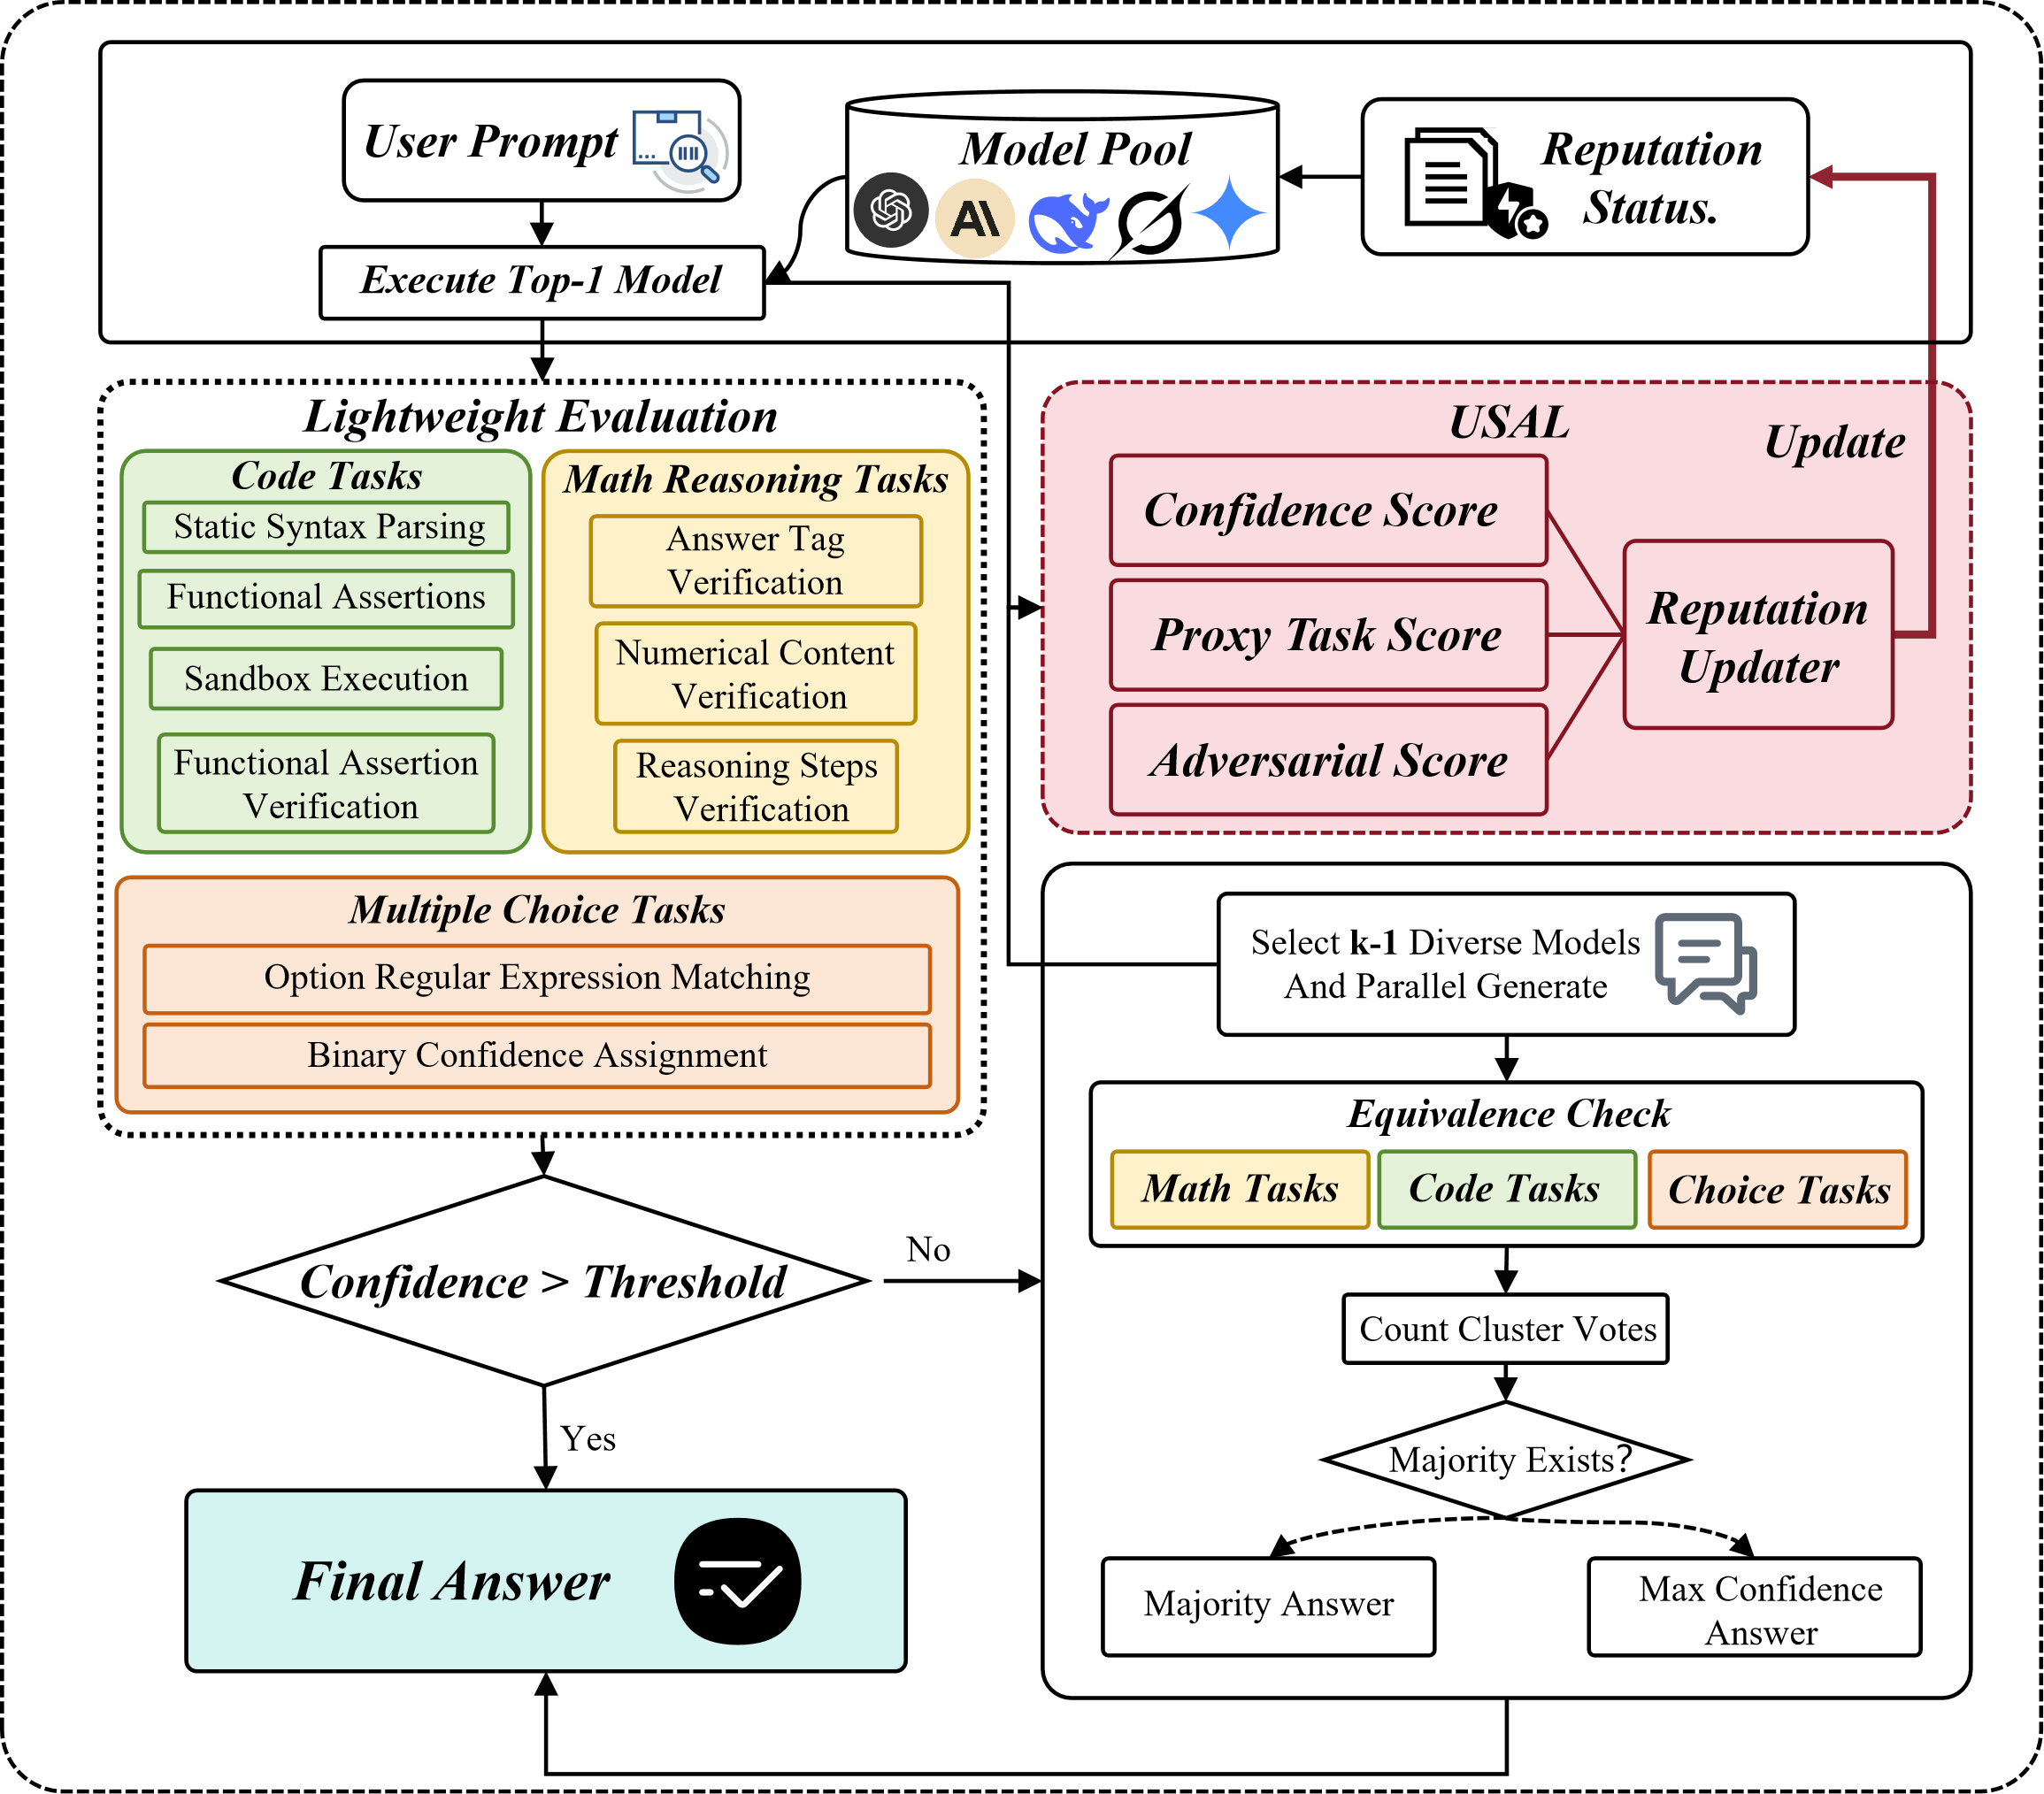
\includegraphics[width=0.8\linewidth]{Pics/图片1.png}
    \caption{Overview of TrustRoute. The middleware first performs a top-1 fast pass with auditable lightweight evaluation; if confidence is insufficient, it escalates to a bounded parallel set and aggregates candidates deterministically. Crucially, auditable feedback (e.g., execution outcomes when available and deterministic proxy checks otherwise) forms a feedback loop: it updates agent reputations via USAL, which in turn affects future utility ranking and routing decisions under model/API drift.}
    \label{fig:trustroute}
\vspace{-0.7cm}
\end{figure}

\subsection{Overview}
\label{sec:overview}
TrustRoute is an inference-time routing middleware for a pool of heterogeneous black-box LLM agents
$\mathcal{A}=\{A_1,\ldots,A_M\}$.
For a user query $x$, querying an agent $A_i$ returns an output $y_i$ together with observable operational signals,
including monetary cost $c_i$ (e.g., API-reported token usage) and wall-clock latency $\ell_i$.
Our goal is to maximize answer reliability while controlling expected cost and latency under model/API drift.

TrustRoute achieves this via three coupled components.
First, it maintains an online state for each agent, including a reputation score $R_i\in[0,1]$ and running estimates of cost/latency.
Second, it uses a cost--latency aware utility ranking to select which agent(s) to query.
Third, it adopts a two-stage routing policy:
a top-1 fast pass that attempts to solve most instances with minimal overhead,
and a bounded escalation step that queries a small additional set in parallel only when necessary.
After each query is processed, TrustRoute updates agent reputations online using USAL (Fig.~\ref{fig:usal}),
which relies only on signals that are reproducible at inference time (e.g., deterministic checks, execution outcomes when available, and local history).

Throughout, TrustRoute uses the following hyperparameters:
$k$ is the maximum number of queried agents per instance (including the fast pass);
$\tau_1$ is the confidence threshold for early stopping;
$\tau_2$ and $m$ control the minimum evidence required to accept a majority under escalation;
$\eta$ is the learning rate for reputation updates; and
$\alpha,\beta$ balance monetary cost versus latency in utility computation.

\subsection{Model Pool and Utility Ranking}
\label{sec:ranking}
TrustRoute requires an ordering over agents to decide (i) which agent to query in the fast pass and (ii) which agents to include upon escalation.
Because agents differ not only in reliability but also in operational overhead, we rank agents by a utility score that approximates
\emph{reliability per unit cost/latency}.

\paragraph{Online agent state.}
For each agent $A_i$, TrustRoute maintains:
(1) an online reputation $R_i\in[0,1]$, updated by USAL (\S\ref{sec:usal});
(2) running estimates of expected monetary cost and latency, denoted by $\bar{c}_i$ and $\bar{\ell}_i$.
We compute $\bar{c}_i$ and $\bar{\ell}_i$ using exponential moving averages over observed per-call measurements,
so estimates remain stable yet responsive to drift:
\[
\bar{c}_i \leftarrow (1-\rho)\bar{c}_i + \rho c_i,\quad
\bar{\ell}_i \leftarrow (1-\rho)\bar{\ell}_i + \rho \ell_i,
\]
for a smoothing factor $\rho\in(0,1)$.

\paragraph{Utility score.}
Given $(R_i,\bar{c}_i,\bar{\ell}_i)$, we compute the utility:
\begin{equation}
U_i = \frac{R_i}{\alpha \bar{c}_i + \beta \bar{\ell}_i + \epsilon},
\label{eq:utility}
\end{equation}
where $\alpha,\beta\ge 0$ control the relative importance of monetary cost versus latency, and $\epsilon>0$ avoids division by zero.
Eq.~\ref{eq:utility} promotes agents that are recently reliable (high $R_i$) and penalizes agents that are expensive or slow.

\paragraph{Selection for fast pass and escalation.}
TrustRoute ranks agents by descending $U_i$.
The fast pass queries the top-ranked agent $A_{i^\star}=\arg\max_i U_i$.
If escalation is triggered, TrustRoute queries up to $(k-1)$ additional agents by continuing down the ranked list.
When metadata is available, the selection can enforce lightweight diversity (e.g., provider diversity) to reduce correlated failures.
To mitigate cold-start volatility, $\bar{c}_i$ and $\bar{\ell}_i$ are conservatively initialized (e.g., pool medians) and updated only from observed calls; similarly, $R_i$ is updated from auditable signals rather than agreement alone (\S\ref{sec:usal}).


\begin{algorithm}[t]
\caption{TrustRoute routing (two-stage with online updates)}
\label{alg:trustroute_short}
\begin{algorithmic}[1]
\Require query $x$ (task family $T$); agent pool $\mathcal{A}$; max agents $k$;
thresholds $\tau_1,\tau_2$; min support $m$
\Ensure answer $\hat{y}$

\State $\pi \gets \Call{RankByUtility}{\mathcal{A}}$; \ $i^\star \gets \pi_1$
\State $(y^\star, z^\star, \gamma^\star) \gets \Call{QueryEval}{i^\star, x, T}$

\Statex \textit{/* Stage 1 (fast pass) */}
\If{$\gamma^\star \ge \tau_1$}
    \State \Call{OnlineUpdate}{$\{i^\star\}, \{(z^\star,\gamma^\star)\}$}
    \State \Return $y^\star$
\EndIf

\Statex \textit{/* Stage 2 (escalation) */}
\State $S \gets \{i^\star\} \cup \Call{TopK}{\pi, k{-}1}$
\ForAll{$i \in S\setminus\{i^\star\}$ \textbf{in parallel}}
    \State $(y_i, z_i, \gamma_i) \gets \Call{QueryEval}{i, x, T}$
\EndFor
\State $V \gets \{z_i \mid i\in S \wedge z_i\neq \bot\}$  \Comment{ignore unextractable keys}
\If{$|V|=0$}
    \State $\hat{i}\gets \arg\max_{i\in S}\gamma_i$  \Comment{fallback when no key is extractable}
    \State \Call{OnlineUpdate}{$S, \{(z_i,\gamma_i)\}_{i\in S}$}
    \State \Return $y_{\hat{i}}$
\EndIf
\State $v^\star \gets \Call{Mode}{V}$

\If{\Call{Consensus}{$\{z_i\}_{i\in S}, v^\star, \tau_2, m$}}
    \State $C \gets \{i\in S: z_i=v^\star\}$; \ $\hat{i}\gets \arg\max_{i\in C}\gamma_i$
\Else
    \State $\hat{i}\gets \arg\max_{i\in S}\gamma_i$
\EndIf
\State \Call{OnlineUpdate}{$S, \{(z_i,\gamma_i)\}_{i\in S}$}
\State \Return $y_{\hat{i}}$
\end{algorithmic}
\end{algorithm}

\subsection{Lightweight Evaluation}
\label{sec:lightweight}
A core requirement in TrustRoute is \emph{auditable early stopping}: the router should return after the fast pass only when it has strong, reproducible evidence that the output is reliable.
To this end, TrustRoute performs lightweight evaluation for each candidate output and produces a confidence score.

\paragraph{Confidence decomposition.}
Given an output $y_i$, TrustRoute computes:
(i) a proxy task score $q_i\in[0,1]$ from fast deterministic checks, and
(ii) an intrinsic consistency score $h_i\in[0,1]$ derived from the agent's recent behavior over a sliding window (e.g., stability/validity rate).
These are combined as:
\begin{equation}
\gamma_i = \lambda q_i + (1-\lambda) h_i,
\label{eq:confidence}
\end{equation}
where $\lambda\in[0,1]$ balances instance-level evidence and short-term stability.

\paragraph{Early-stopping rule.}
After the fast-pass agent produces $(y_1,\gamma_1)$, TrustRoute returns immediately if $\gamma_1 \ge \tau_1$; otherwise it escalates.
This design ensures the decision to stop early is driven by a reproducible confidence estimate rather than opaque heuristics.

\paragraph{Proxy task score $q_i$ by task family.}
TrustRoute instantiates $q_i$ with task-aware checks that are fast and deterministic.

\textbf{Executable code tasks.}
We run static checks (e.g., syntax parsing) and sandbox execution with timeouts.
When unit tests or fixed I/O checks are available, we use the strong oracle outcome
$\mathsf{Exec}(y_i)\in\{\textsc{pass},\textsc{fail},\textsc{error/timeout}\}$ and map it to:
\begin{equation}
q_i=
\begin{cases}
1.0, & \mathsf{Exec}(y_i)=\textsc{pass},\\
0.6, & \mathsf{Exec}(y_i)=\textsc{fail},\\
0.0, & \mathsf{Exec}(y_i)=\textsc{error/timeout}.
\end{cases}
\label{eq:score_exec}
\end{equation}
We assign a non-zero score to \textsc{fail} because runnable code is typically closer to a correct solution than \textsc{error/timeout}: it preserves syntactic validity and executable structure, and is often fixable by minor edits or by other agents during escalation.
In contrast, \textsc{error/timeout} indicates non-executability or instability, providing weaker evidence of correctness.

\textbf{Math reasoning tasks.}
We deterministically extract the final answer (e.g., normalized numeric/string span) and validate its format (units, separators, sign).
When intermediate constraints are present (e.g., explicit equations or bounds), we apply lightweight consistency checks.
The score $q_i$ rewards successful extraction and consistency; malformed or missing answers are penalized.

\textbf{Multiple-choice tasks.}
We extract the selected option using regular expressions and enforce validity against the option set.
Outputs with ambiguous or missing selections receive lower $q_i$.

\paragraph{Intrinsic consistency score $h_i$.}
To respond quickly to drift (e.g., increased timeout rate or formatting instability), TrustRoute maintains a short sliding window per agent.
We compute $h_i$ deterministically from recent outcomes (e.g., proportion of valid extractions, crash/timeout frequency, recent execution stability).
As a result, an agent that becomes unstable receives reduced confidence even before many failures accumulate in $R_i$.

\subsection{Equivalence Check}
\label{sec:voting}
When the fast pass confidence is insufficient, TrustRoute escalates to query up to $(k-1)$ additional agents in parallel and then aggregates their outputs.
The aggregation is designed to be deterministic and robust to heterogeneous output formats.

\paragraph{Parallel querying.}
Upon escalation, TrustRoute selects additional agents from the utility-ranked list (Eq.~\ref{eq:utility}) and obtains $k$ candidate outputs $\{y_1,\ldots,y_k\}$.
For each candidate, it computes the confidence score $\gamma_j$ using the same lightweight evaluation pipeline (\S\ref{sec:lightweight}).

\paragraph{Equivalence keys and clustering.}
To compare heterogeneous outputs, TrustRoute uses a task-dependent key extractor $\kappa(\cdot)$ and sets
$z_j=\kappa(y_j)\in\mathcal{Z}\cup\{\bot\}$, where $\bot$ denotes an unextractable key.
Keys represent answer identity under normalization (e.g., normalized numeric answers for math, option IDs for choice).
For code tasks, keys can be derived from auditable execution signatures when available (e.g., pass/fail plus failing test identifiers), or from deterministic structural signatures otherwise.
We cluster candidates by key equality and count cluster votes.

\paragraph{Agreement rate and minimum-support rule.}
Let $v^\star$ be the key with the most votes among defined keys.
We define the agreement rate with a fixed denominator $k$:
\begin{equation}
p = \max_v \frac{\sum_{j=1}^{k}\mathbb{I}[z_j=v]}{k}.
\label{eq:agreement}
\end{equation}
TrustRoute accepts a majority only when it has sufficient support:
\begin{equation}
p \ge \tau_2 \ \ \text{and}\ \ \sum_{j=1}^{k}\mathbb{I}[z_j=v^\star]\ge m.
\label{eq:min_support}
\end{equation}
This prevents spurious ``agreement'' caused by a single extractable output or missing keys.
\paragraph{\textsc{Consensus} definition.}
Given the majority key $v^\star$, we define the support $s=\sum_{i\in S}\mathbb{I}[z_i=v^\star]$ and the agreement rate $p=s/k$,
where $k=|S|$ is the number of queried agents (fixed denominator to penalize unextractable keys).
\textsc{Consensus} returns \textbf{true} iff $p\ge\tau_2$ and $s\ge m$; otherwise it returns \textbf{false}.



\paragraph{Selection rule.}
If Eq.~\ref{eq:min_support} holds, TrustRoute returns a representative from the majority cluster, preferring the candidate with the highest confidence $\gamma_j$ within that cluster.
If no majority satisfies the rule, TrustRoute returns the max-confidence candidate $\arg\max_j \gamma_j$; utility $U_i$ is used only as a tie-breaker.
This prioritizes auditable instance-level evidence during aggregation while remaining resource-aware through the selection policy.









\subsection{USAL: Online Reputation Update from Auditable Signals}
\label{sec:usal}



\begin{figure}[t]
    \centering
    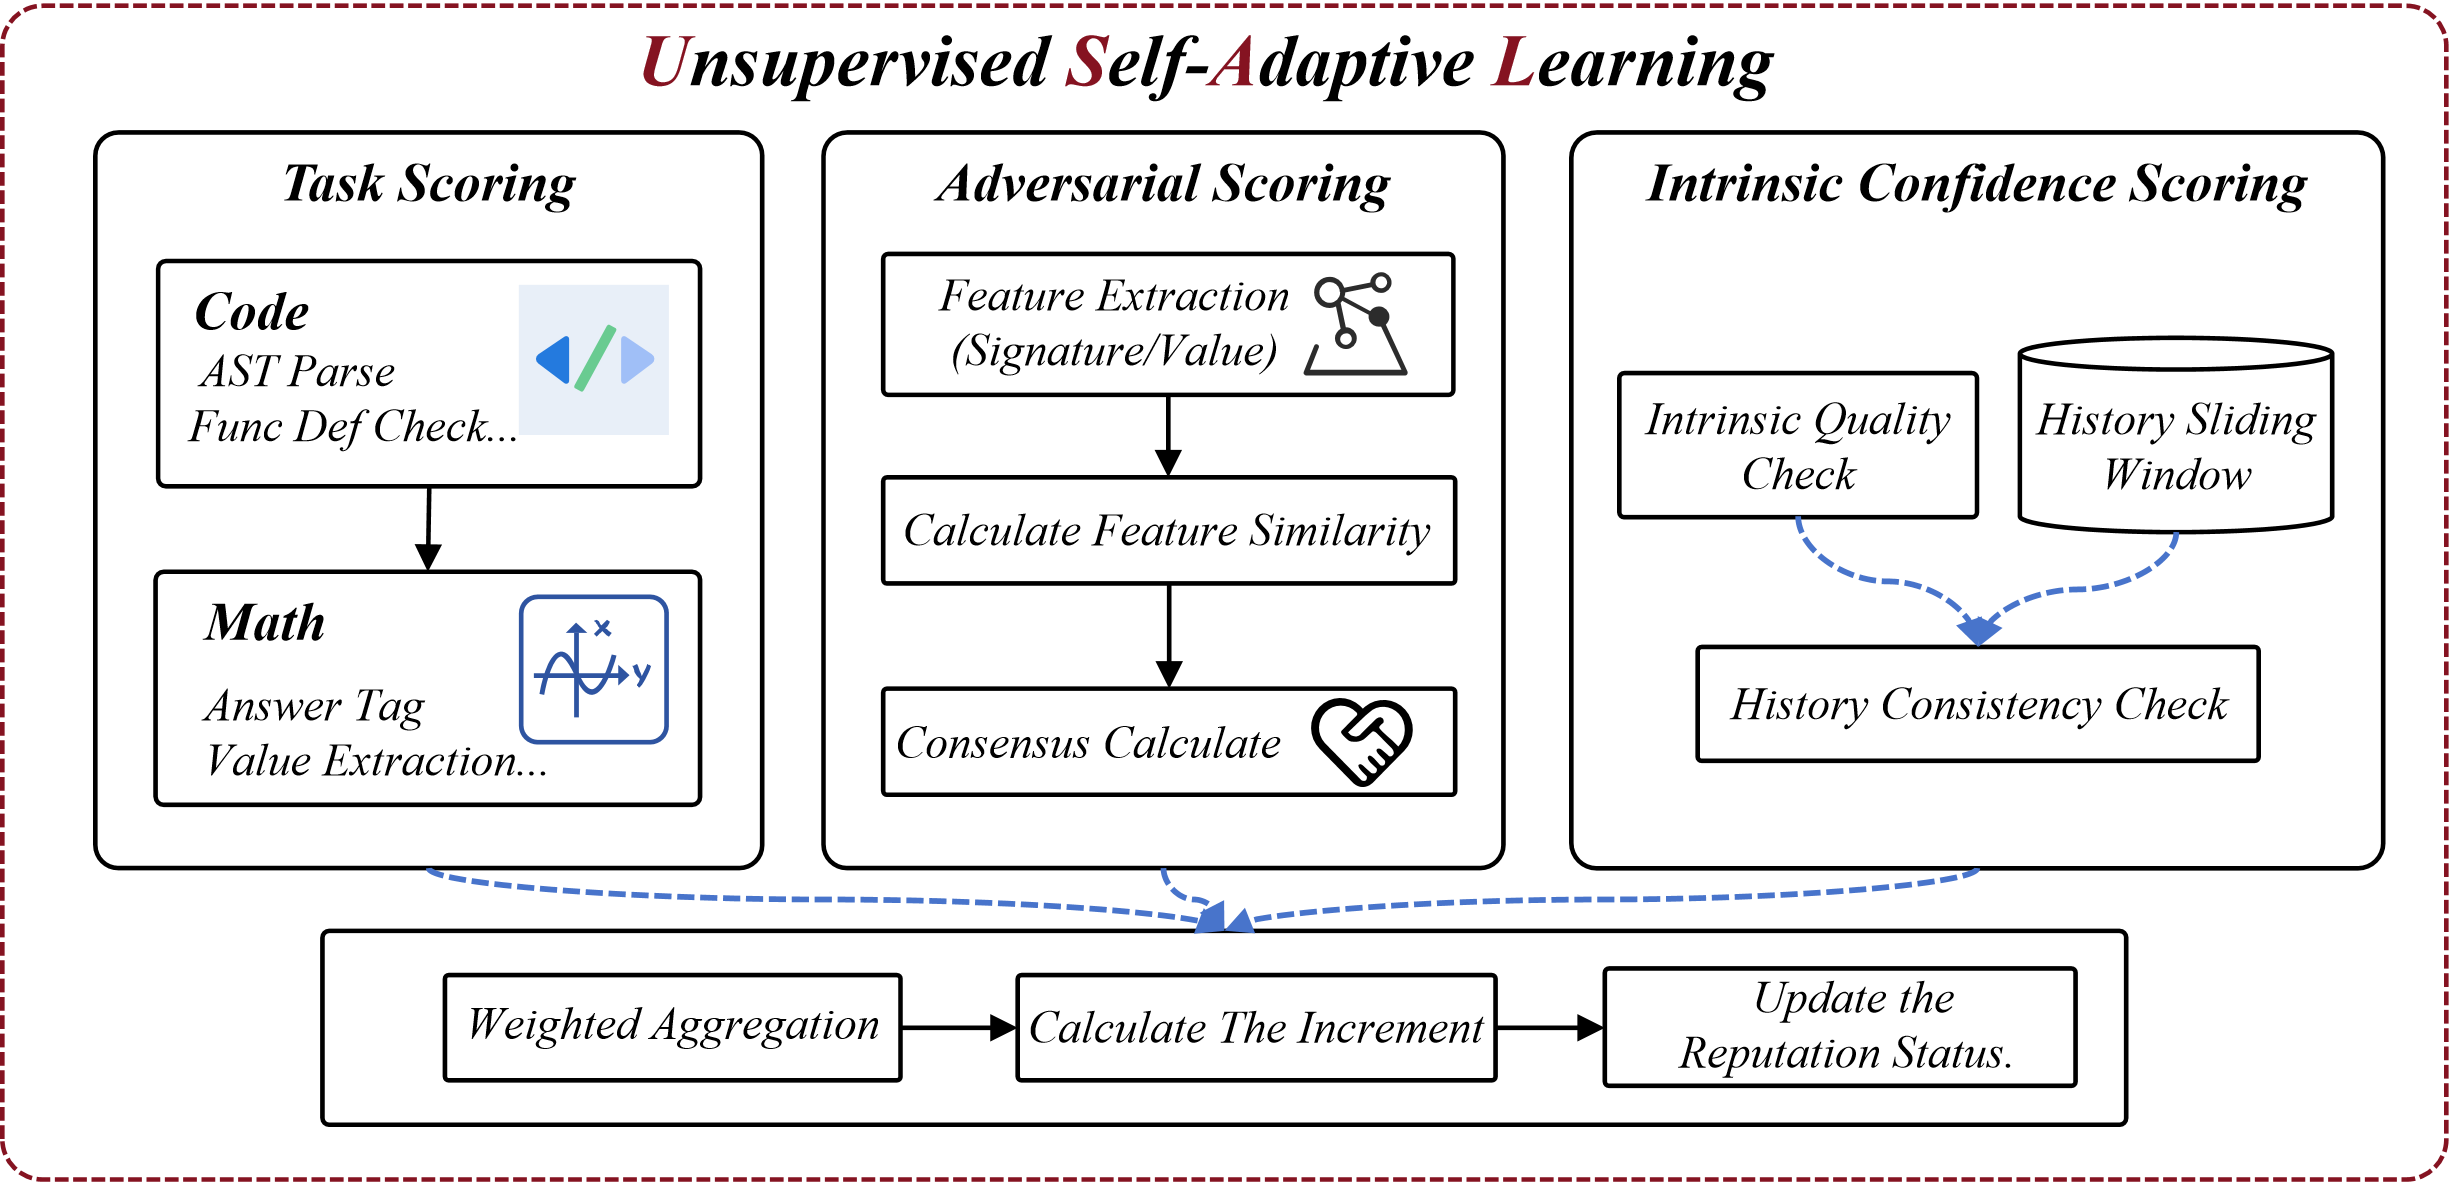
\includegraphics[width=0.8\linewidth]{Pics/图片2.png}
    \caption{Overview of USAL. USAL updates agent reputations using auditable signals from task scoring, cross-agent agreement scoring, and intrinsic history-based stability.}

    \label{fig:usal}
\end{figure}

TrustRoute updates agent reputations online using USAL.
USAL is ``unsupervised'' in the operational sense that it requires no human labels and no offline retraining: all update signals are computed deterministically at inference time from auditable checks and local histories.
The objective is to maintain a drift-adaptive reliability estimate $R_i$ that is stable, responsive, and not overly dependent on agreement.

\paragraph{Signal design.}
For each queried agent $A_i$ at round $t$, USAL computes three normalized signals in $[0,1]$.

\textbf{Task score $q_i^{(t)}$.}
USAL uses the proxy task score produced by lightweight evaluation (\S\ref{sec:lightweight}).
For executable code tasks, $q_i^{(t)}$ is instantiated by Eq.~\ref{eq:score_exec}, which is directly auditable.

\textbf{Agreement score $a_i^{(t)}$ (cross-agent consistency).}
USAL uses a simple, fully deterministic agreement signal to capture whether an agent's extracted key aligns with others.
Given the queried set $S$ and extracted keys $\{z_j\}_{j\in S}$, we define
\[
a_i^{(t)} = \mathbb{I}[z_i\neq\bot]\cdot \frac{1}{|S|}\sum_{j\in S}\mathbb{I}[z_j=z_i].
\]
When $|S|=1$ (fast pass without escalation), we set $a_i^{(t)}$ to a constant prior $a_0$.
This term is \emph{not} an adversarial detector; it is a lightweight consensus indicator that is reproducible and label-free.


\textbf{Intrinsic consistency $h_i^{(t)}$ (history-based).}
USAL maintains a short sliding window of recent agent behaviors (e.g., validity rates, crash/timeout frequency, execution stability) and converts it into a score $h_i^{(t)}$.
This ensures reputations react quickly when an agent becomes unstable due to drift.

\paragraph{Weighted aggregation and EMA update.}
USAL aggregates these auditable signals:
\begin{equation}
s_i^{(t)} = w_q q_i^{(t)} + w_a a_i^{(t)} + w_h h_i^{(t)},
\label{eq:usal_score}
\end{equation}
where $w_q,w_a,w_h\ge0$ and $w_q+w_a+w_h=1$.
It then updates the reputation with an exponential moving average:
\begin{equation}
R_i^{(t)} = (1-\eta)R_i^{(t-1)} + \eta \cdot s_i^{(t)}.
\label{eq:ema}
\end{equation}
This update yields a smooth estimate of recent reliability while remaining responsive to drift.
Importantly, because $s_i^{(t)}$ is grounded in auditable task evidence, deterministic robustness proxies, and history stability, it avoids self-reinforcing reputations based solely on inter-model agreement, which can be misleading under correlated failures.
\begin{algorithm}[H]
\caption{USAL: online reputation update from auditable signals}
\label{alg:usal}
\begin{algorithmic}[1]
\Require \parbox[t]{0.93\linewidth}{
queried set $S$; keys $\{z_i\}_{i\in S}$; per-agent signals $\{(q_i,h_i)\}_{i\in S}$\\
reputations $\{R_i\}$ and histories $\{H_i\}$; weights $w_q,w_a,w_h$; learning rate $\eta$; window $W$; prior $a_0$
}
\Ensure updated $\{R_i,H_i\}$

\State $k \gets |S|$
\ForAll{$i\in S$}
    \If{$k=1$}
        \State $a_i \gets a_0$
    \Else
        \State $a_i \gets \mathbb{I}[z_i\neq\bot]\cdot \frac{1}{k}\sum_{j\in S}\mathbb{I}[z_j=z_i]$
    \EndIf
    \State $s_i \gets w_q q_i + w_a a_i + w_h h_i$
    \State $R_i \gets (1-\eta)R_i + \eta\cdot s_i$
    \State $H_i \gets \Call{UpdateHistory}{H_i,(q_i,a_i),W}$
\EndFor
\State \Return
\end{algorithmic}
\end{algorithm}
\section{Experiment Setup}
\label{sec:exp_setup}

\subsection{Datasets \& Models}
\label{sec:exp_data_models}

\textbf{Datasets.}
We evaluate TrustRoute on seven widely-used benchmarks spanning code generation, mathematical reasoning, and multiple-choice commonsense/knowledge reasoning:
\textbf{HumanEval} (164) and \textbf{MBPP} (378) for code generation with executable unit tests,
\textbf{GSM8K} (1{,}319) for multi-step math reasoning,
and \textbf{ARC-Challenge} (1{,}172), \textbf{HellaSwag}, \textbf{MMLU}, and \textbf{Winogrande} (1{,}267) for multiple-choice reasoning.
For \textbf{HellaSwag} and \textbf{MMLU}, we use a \emph{deterministic subset of the first 1,000 instances} from the official test split to manage commercial API costs; for all other benchmarks, we evaluate on the \emph{full official test split}.
The exact instance IDs used for the HellaSwag/MMLU subsets are provided in the artifact for reproducibility.


\textbf{Models.}
TrustRoute routes each query to a heterogeneous pool of black-box LLM agents accessed via a unified API gateway.
We use a dedicated \emph{judge} model for lightweight verification/scoring signals when needed, and a candidate pool for answering.
Unless a baseline inherently requires sampling (e.g., self-consistency), we use fixed inference parameters across methods.
Table~\ref{tab:model_pool} summarizes the agent pool used in our experiments, including the model identifier,
decoding parameters, and the pricing/latency snapshot used for cost accounting.
We compare TrustRoute against representative routing and ensembling baselines:
\textbf{SA} (single-agent greedy decoding);
\textbf{SC-$k$} (self-consistency majority vote with $k\in\{3,5,10\}$) \cite{wang2023selfconsistency};
\textbf{FrugalGPT (variant)} (training-free heuristic cascading) \cite{chen2023frugalgpt};
\textbf{Cascade} (a cost-sorted fixed-order fallback chain that sequentially escalates to stronger/more expensive agents);
\textbf{MV-3} (three-way parallel voting without adaptivity);
and \textbf{Random} (uniformly sampling from the same candidate set).
For fairness, all baselines draw candidates from the same agent pool and share the same prompting template.

\textbf{Training-free implementations.}
All baselines are implemented without any additional router/verifier training.
In particular, \textbf{FrugalGPT (variant)} follows the cascade-style policy in~\cite{chen2023frugalgpt} but \emph{omits the learned scorer/discriminator}, since training a task-specific routing classifier is impractical in our zero-shot black-box API setting.
Concretely, it \emph{cascades models by increasing cost} and stops early when a candidate passes deterministic validity checks (e.g., parsable/answer-extractable; executable when applicable).
Similarly, \textbf{Cascade} is a purely heuristic baseline that \emph{sequentially escalates along the same cost-sorted order} without adaptivity or online learning.
\begin{table}[H]
\centering
\caption{Model pool used in our experiments. \textbf{Units:} Prompt/Comp.\ are USD per 1K tokens. We use this pricing snapshot for cost accounting; actual latency is measured as wall-clock time per request.}
\label{tab:model_pool}
\small
\setlength{\tabcolsep}{6pt}
\begin{tabular}{l c c r r r}
\toprule
\textbf{Model} & \textbf{Role} & \textbf{Temp} & \textbf{MaxTok} & \textbf{Prompt} & \textbf{Comp.} \\
\midrule
claude-haiku-4-5-20251001      & judge & 0.0 & 1024 & 0.00100 & 0.00500 \\
\midrule
gpt-4o-mini                    & cand. & 0.2 & 1024 & 0.00015 & 0.00060 \\
gpt-5-mini                     & cand. & 0.2 & 1024 & 0.00025 & 0.00200 \\
gemini-2.5-flash               & cand. & 0.2 & 1024 & 0.00030 & 0.00250 \\
claude-sonnet-4-5-20250929     & cand. & 0.2 & 1024 & 0.00300 & 0.01500 \\
grok-3-mini                    & cand. & 0.2 & 1024 & 0.00030 & 0.00050 \\
deepseek-r1                    & cand. & 0.2 & 1024 & 0.00055 & 0.00248 \\
\bottomrule
\end{tabular}
\end{table}


\subsection{Metrics}
\label{sec:exp_metrics}
We report \textbf{Accuracy} (fraction of tasks solved correctly), \textbf{Cost} (USD per query), and \textbf{Latency} (seconds per query), averaged over all evaluated instances.
And we also introduce the \textbf{J} to evaluate the overall trade-off: $J = \frac{1}{3} [ \hat{Acc} + (1-\hat{Cost}) + (1-\hat{Lat}) ] \times 100$, where the metrics are min--max normalized \emph{per dataset across the compared methods in the same table}.
As a result, the absolute value of $J$ depends on the method set in that table and is intended for \textbf{within-table} comparisons; for cross-table comparison we rely on raw Acc/Cost/Lat.


\subsection{Evaluation Protocol}
\label{sec:exp_protocol}
\textbf{Hyperparameter tuning.}TrustRoute involves routing hyperparameters, including confidence thresholds $(\tau_1,\tau_2)$,
USAL weights $\mathbf{w}=(w_q,w_a,w_h)$, utility coefficients $(\alpha,\beta)$, and a minimum reputation constraint.

To mitigate test-set overfitting, we perform model selection on a small development subset:
for each benchmark, we randomly sample \textbf{10\%} of the evaluation split using a fixed sampling seed,
select the best configuration under our selection criterion (e.g., accuracy subject to a budget),
and then report final results on the remaining \textbf{90\%} instances.



\textbf{Repeated runs and reporting.}
Unless otherwise stated, we repeat each method with three independent random seeds
$\{1,2,3\}$ and report the mean and standard deviation across runs.
For TrustRoute and other adaptive methods, the seed controls both the stochastic components in routing
(e.g., exploration) and any randomness in evaluation sub-sampling; non-adaptive baselines typically exhibit
near-zero variance under deterministic decoding.

\textbf{Run isolation.}
TrustRoute maintains an online reputation state during inference.
To prevent cross-run interference (especially under parallel execution), we isolate the reputation cache
by \texttt{(dataset, seed)} so that each run starts from a clean state and updates only its own cache.





\section{Results and Analysis}

\subsection{RQ1: Overall Effectiveness}




\begin{table*}[t]
\centering
\footnotesize
\setlength{\tabcolsep}{2.0pt} % 稍微收紧列间距以适应科学计数法
\renewcommand{\arraystretch}{1.12}
\caption{Main results on 7 datasets. Cost is shown in scientific notation (e.g., 2.66e-4 = \$0.000266). GSM8K results updated. (Acc/J in \%, Lat in s).}
\label{tab:main_results}
\begin{tabular}{lcccc cccc cccc cccc}
\toprule
\multirow{2}{*}{\textbf{Method}} &
\multicolumn{4}{c}{\textbf{HumanEval}} &
\multicolumn{4}{c}{\textbf{MBPP}} &
\multicolumn{4}{c}{\textbf{GSM8K}} &
\multicolumn{4}{c}{\textbf{ARC}} \\
\cmidrule(lr){2-5}\cmidrule(lr){6-9}\cmidrule(lr){10-13}\cmidrule(lr){14-17}
& Acc & Cost & Lat & J & Acc & Cost & Lat & J & Acc & Cost & Lat & J & Acc & Cost & Lat & J \\
\midrule
SA                  & 86.3 & \textbf{2.66e-4} & \textbf{6.39}  & 66.7 & 87.1 & \textbf{1.52e-4} & 4.05  & 66.4 & \textbf{90.9} & \textbf{2.04e-4} & \textbf{5.35}  & \textbf{100.0} & 91.4 & \textbf{2.10e-5} & \textbf{1.05} & 66.9 \\
SC\textendash{}3    & 86.5 & 7.99e-4          & 20.17          & 55.4 & 87.8 & 4.46e-4          & 12.71 & 61.2 & 88.6 & 5.68e-4          & 14.49          & 81.7 & 91.6 & 6.40e-5          & 3.19          & 66.3 \\
SC\textendash{}5    & 87.0 & 1.33e-3          & 40.81          & 38.6 & 87.0 & 7.43e-4          & 20.63 & 47.9 & 85.0 & 9.46e-4          & 23.08          & 59.9 & 92.0 & 1.07e-4          & 5.39          & 66.1 \\
SC\textendash{}10   & \textbf{98.9} & 2.67e-3          & 46.81          & 66.0 & 90.0 & 1.49e-3          & 33.92 & 45.1 & 89.2 & 1.89e-3          & 42.81          & 47.1 & 91.6 & 2.13e-4          & 10.88         & 61.9 \\

FrugalGPT           & 93.0 & 2.09e-3          & 24.61          & 61.9 & 92.7 & 7.53e-4          & 13.83 & 86.5 & 80.1 & 3.86e-4          & 11.33          & 59.9 & 97.1 & 2.64e-4          & 4.57          & 98.2 \\
Cascade             & 95.3 & 9.38e-4          & 19.68          & 76.9 & \textbf{92.8} & 7.29e-4          & 23.77 & 76.0 & 82.3 & 4.59e-4          & 9.89           & 67.3 & 96.9 & 3.87e-3          & 81.50         & 33.3 \\
MV\textendash{}3    & 95.5 & 1.12e-2          & 30.10          & 38.2 & 88.7 & 8.61e-3          & 28.82 & 15.3 & 84.8 & 4.20e-3          & 26.52          & 29.2 & 96.9 & 1.96e-3          & 35.96         & 68.6 \\
Random              & 95.0 & 4.08e-3          & 11.53          & 67.5 & 89.0 & 2.83e-3          & 12.59 & 56.5 & 84.3 & 1.36e-3          & 7.56           & 68.0 & 96.6 & 6.30e-4          & 11.32         & 89.9 \\

\textbf{TrustRoute} & 97.7 & 2.27e-3 & 8.24  & \textbf{89.3} & 91.4 & 1.65e-3          & \textbf{3.82}  & \textbf{86.3} & 88.7 & 2.60e-3          & 12.10          & 67.3 & \textbf{97.3} & 2.26e-4          & 2.11          & \textbf{98.3} \\
\bottomrule
\end{tabular}

\vspace{8pt}

\begin{tabular}{lcccc cccc cccc}
\toprule
\multirow{2}{*}{\textbf{Method}} &
\multicolumn{4}{c}{\textbf{HellaSwag}} &
\multicolumn{4}{c}{\textbf{MMLU}} &
\multicolumn{4}{c}{\textbf{Winogrande}} \\
\cmidrule(lr){2-5}\cmidrule(lr){6-9}\cmidrule(lr){10-13}
& Acc & Cost & Lat & J & Acc & Cost & Lat & J & Acc & Cost & Lat & J \\
\midrule
SA                  & 70.7 & \textbf{4.00e-5} & \textbf{1.10} & 67.3 & 72.4 & \textbf{2.90e-5} & \textbf{1.12} & 66.7 & 71.4 & \textbf{1.60e-5} & \textbf{1.06} & 67.9 \\
SC\textendash{}3    & 70.4 & 1.19e-4          & 3.30          & 66.3 & 73.0 & 8.80e-5          & 3.43          & 67.4 & 70.8 & 4.70e-5          & 3.23          & 66.7 \\
SC\textendash{}5    & 70.1 & 1.98e-4          & 5.49          & 65.5 & 73.0 & 1.52e-4          & 5.77          & 67.1 & 70.5 & 7.90e-5          & 5.41          & 66.2 \\
SC\textendash{}10   & 71.1 & 3.96e-4          & 11.07         & 64.9 & 72.3 & 2.93e-4          & 11.34         & 64.5 & 70.6 & 1.58e-4          & 10.82         & 64.3 \\

FrugalGPT           & 76.6 & 5.43e-4          & 9.15          & 70.9 & 84.5 & 2.74e-4          & 9.01          & 86.8 & 87.2 & 2.86e-4          & 5.76          & 90.1 \\
Cascade             & 95.0 & 6.57e-3          & 89.02         & 32.3 & 79.0 & 5.60e-3          & 95.94         & 12.3 & \textbf{91.3} & 3.90e-3          & 91.27         & 33.3 \\
MV\textendash{}3    & 85.5 & 3.28e-3          & 40.75         & 51.6 & 87.0 & 2.94e-3          & 47.49         & 59.9 & 89.0 & 1.89e-3          & 54.27         & 60.1 \\
Random              & 80.9 & 9.78e-4          & 9.14          & 74.4 & 84.3 & 8.17e-4          & 9.74          & 85.6 & 86.6 & 5.58e-4          & 11.63         & 87.9 \\

\textbf{TrustRoute} & \textbf{95.7} & 1.09e-3          & 2.98          & \textbf{94.0} & \textbf{90.2} & 1.49e-3          & 3.19          & \textbf{90.5} & 88.3 & 1.07e-3          & 3.46          & \textbf{91.3} \\
\bottomrule
    \end{tabular}
\end{table*}



Table~\ref{tab:main_results} reports results on seven benchmarks spanning code generation (HumanEval, MBPP), math reasoning (GSM8K), and knowledge/commonsense multiple-choice tasks (ARC-Challenge, HellaSwag, MMLU, Winogrande).
To quantify the effectiveness--efficiency trade-off, we report \emph{J-Score}, which aggregates accuracy, cost, and latency into a unified metric.\footnote{We follow the J-Score definition in Sec.~\ref{sec:exp_metrics}.}
Overall, TrustRoute achieves the best J-Score on six datasets (HumanEval, HellaSwag, MMLU, Winogrande, and ARC-Challenge), remains highly competitive on MBPP, and shows limited benefit on GSM8K where the base model is already strong.

On code generation, TrustRoute improves reliability without relying on uniformly expensive sampling.
On HumanEval, TrustRoute attains a J-Score of 89.3, substantially exceeding large-sampling self-consistency SC-10 (66.0).
Although SC-10 reaches slightly higher accuracy (98.9\%), it incurs much higher cost and latency, which weakens its aggregate trade-off.
In contrast, TrustRoute maintains comparable accuracy (97.7\%) with markedly lower latency (8.24s vs.\ 46.81s), indicating that verification-aware routing can produce more efficient reliability gains than simply increasing sample count.
On MBPP, TrustRoute achieves a J-Score of 86.3 with 91.4\% accuracy and low latency (3.82s), closely matching the strongest efficiency-oriented baseline, suggesting that the two-stage policy generalizes across different programming distributions.

On knowledge and commonsense reasoning, TrustRoute consistently achieves strong J-Scores across multiple-choice tasks.
For instance, on HellaSwag it reaches 95.7\% accuracy and a J-Score of 94.0, compared to 67.3 for the single-agent baseline (SA).
On MMLU and Winogrande, TrustRoute similarly leads in J-Score while operating at low latency (3.19s and 3.46s).
Compared to heavy multi-agent pipelines such as Cascade, TrustRoute achieves comparable or better accuracy at orders-of-magnitude lower latency on some tasks, consistent with its design goal: Stage~1 resolves most instances cheaply, while Stage~2 is reserved for the uncertain tail.

GSM8K is the main exception.
TrustRoute obtains a J-Score of 67.3, below SA (100.0).
This gap is consistent with a near-saturated regime: SA already reaches 90.9\% accuracy on GSM8K, leaving limited headroom for routing-based gains.
Moreover, conservative confidence gating can trigger unnecessary Stage~2 escalation for instances that are solvable by a single agent, increasing cost ($2.60e^{-3}$) and latency (12.10\,s) with limited accuracy improvement.
These results suggest that when the base model is already strong, controlling false-positive escalations (e.g., via calibration or task-specific thresholds) is critical to avoid overhead-dominated operating points.

\begin{findingbox}
\textbf{Finding 1:} \textit{Selective escalation guided by verification-aware confidence yields a consistently better reliability--efficiency frontier than uniformly expensive sampling or always-on multi-agent querying across diverse tasks; the largest gains arise when the base model has meaningful headroom, while near-saturated regimes require tighter escalation control to prevent overhead without returns.}
\end{findingbox}





\begin{table*}[t]
\centering
\footnotesize
\setlength{\tabcolsep}{2.4pt}
\renewcommand{\arraystretch}{1.12}
\caption{\textbf{Ablation of TrustRoute components.} Acc in \%, Cost in \$/query, Lat in seconds. We also report $J$ (higher is better), where Acc/Cost/Lat are min-max normalized per dataset across the variants in this table.
\textbf{Variant legend:} \textbf{w/o Cost obj.} removes the cost term from the routing objective; \textbf{w/o Cost rank.} disables cost-aware candidate ranking; \textbf{w/o Parallel esc.} disables parallel escalation (forces single-candidate execution); \textbf{w/o Rep. update} disables online reputation updating.}
\label{tab:ablation}

\begin{tabular}{lcccc cccc cccc cccc}
\toprule
\multirow{2}{*}{\textbf{Variant}} &
\multicolumn{4}{c}{\textbf{HumanEval}} &
\multicolumn{4}{c}{\textbf{MBPP}} &
\multicolumn{4}{c}{\textbf{GSM8K}} &
\multicolumn{4}{c}{\textbf{ARC}} \\
\cmidrule(lr){2-5}\cmidrule(lr){6-9}\cmidrule(lr){10-13}\cmidrule(lr){14-17}
& Acc & Cost & Lat & J & Acc & Cost & Lat & J & Acc & Cost & Lat & J & Acc & Cost & Lat & J \\
\midrule
TrustRoute             & 97.7 & 2.27e-3 & 8.24 & 32.1 & 91.4 & 1.65e-3 & 3.82 & 56.1 & 88.7 & 2.60e-3 & 12.10 & 33.3 & 97.1 & 2.26e-4 & 2.11 & 83.8 \\
w/o Cost obj.          & 98.2 & 2.67e-4 & 5.52 & 88.4 & 90.5 & 1.49e-4 & 3.02 & 65.0 & 88.2 & 2.29e-3 & 11.11 & 48.9 & 91.6 & 3.40e-5 & 1.13 & 89.9 \\
w/o Cost Rank.  & 86.3 & 5.24e-4 & 2.24 & 52.2 & 93.5 & 1.26e-3 & 3.62 & 76.4 & 88.2 & 2.29e-3 & 11.08 & 49.7 & 91.6 & 3.31e-5 & 1.15 & 89.4 \\
w/o Parallel esc.      & 85.8 & 8.24e-5 & 1.38 & 66.7 & 91.3 & 2.60e-3 & 4.99 & 26.5 & 85.8 & 1.83e-4 & 5.49 & 66.7 & 91.6 & 2.13e-5 & 1.07 & 93.3 \\
w/o Rep. update        & 88.7 & 7.84e-4 & 3.20 & 61.4 & 93.5 & 1.39e-3 & 3.69 & 68.0 & 88.1 & 2.28e-3 & 11.08 & 50.2 & 91.4 & 1.34e-3 & 4.22 & 0.0 \\
\bottomrule
\end{tabular}

\vspace{8pt}

\begin{tabular}{lcccc cccc cccc}
\toprule
\multirow{2}{*}{\textbf{Variant}} &
\multicolumn{4}{c}{\textbf{HellaSwag}} &
\multicolumn{4}{c}{\textbf{MMLU}} &
\multicolumn{4}{c}{\textbf{Winogrande}} \\
\cmidrule(lr){2-5}\cmidrule(lr){6-9}\cmidrule(lr){10-13}
& Acc & Cost & Lat & J & Acc & Cost & Lat & J & Acc & Cost & Lat & J \\
\midrule
TrustRoute             & 95.7 & 1.09e-3 & 2.98 & 83.6 & 90.2 & 1.49e-3 & 3.19 & 71.7 & 88.3 & 1.07e-3 & 3.46 & 66.6 \\
w/o Cost obj.          & 71.9 & 2.93e-3 & 10.89 & 1.0 & 72.6 & 3.59e-4 & 2.33 & 58.0 & 71.5 & 6.72e-5 & 1.32 & 64.7 \\
w/o Cost Rank.   & 71.2 & 2.90e-3 & 10.92 & 0.3 & 72.6 & 3.75e-4 & 2.35 & 57.7 & 71.7 & 6.65e-5 & 1.32 & 65.1 \\
w/o Parallel esc.      & 71.3 & 3.95e-5 & 1.82 & 66.8 & 72.9 & 2.93e-5 & 1.35 & 67.6 & 71.4 & 1.58e-5 & 1.11 & 66.7 \\
w/o Rep. update        & 71.5 & 2.91e-3 & 10.84 & 0.8 & 72.4 & 2.49e-3 & 8.59 & 0.0 & 71.5 & 1.60e-3 & 8.10 & 0.1 \\
\bottomrule
\end{tabular}
\end{table*}

\subsection{RQ2: Ablation Study}
\label{sec:rq2}

To understand the contribution of each component, Table~\ref{tab:ablation} reports an ablation study that removes (i) cost terms in the routing objective, (ii) cost-aware candidate ranking, (iii) parallel escalation, and (iv) online reputation updating.
We report accuracy, cost, latency, and $J$, where Acc/Cost/Lat are min--max normalized \emph{per dataset across the ablation variants} (as described in the table caption) to highlight the relative impact of design choices.

The ablations indicate that TrustRoute's gains emerge from a coupled design rather than a single heuristic.
Disabling parallel escalation typically pushes the system toward a single-agent regime: the router loses the ability to leverage disagreement across candidates and to select answers supported by multiple agents on ambiguous instances.
Since Stage~2 is triggered on uncertainty, removing parallelism disproportionately affects the hard tail where multiple diverse candidates provide the most leverage.

Removing online reputation updating reduces the router's ability to adapt to drifting agent quality.
In a black-box setting where model/API behavior can change over time, reputation updates provide a mechanism to down-weight agents that have recently been unreliable under the current workload, preventing persistent misrouting.
Without this adaptation, the router is more likely to repeatedly choose suboptimal agents even when auditable feedback indicates quality degradation.

Finally, removing cost-awareness does not necessarily collapse raw accuracy, but it often shifts TrustRoute to a less favorable cost/latency regime.
% This suggests that cost-aware ranking primarily governs where the system lands on the efficiency frontier, preventing the routing policy from implicitly drifting toward an ``always escalate'' behavior that buys reliability by consistently paying for expensive routes.
\begin{findingbox}
\textbf{Finding 2:} \textit{TrustRoute's improvements arise from a coupled design that allocates extra computation only to uncertain instances, continually re-estimates agent trustworthiness from auditable feedback under drift, and explicitly constrains efficiency; parallel escalation and reputation updating account for most reliability gains, while cost-awareness prevents collapse into an always-expensive regime.}
\end{findingbox}
\subsection{RQ3: Hyperparameter Sensitivity and Robustness}
\label{sec:rq3}
We study how sensitive TrustRoute is to key hyperparameters, and whether it exhibits a stable accuracy--cost--latency trade-off under reasonable perturbations.
Specifically, we vary one knob at a time while keeping all others fixed at the default setting:
(i) confidence thresholds $(\tau_1,\tau_2)$, and
(ii) USAL weights $\mathbf{w}=(w_q,w_a,w_h)$ balancing task evidence, cross-agent agreement, and history-based stability.

We report accuracy (\%), cost (\$/query), and latency (s) on dev sets, with $\min\_rep=0$.

Table~\ref{tab:ablate-arcchallenge} shows the results for ARC-Challenge, a representative task illustrating the system's behavioral trends.
Thresholds primarily reshape the control flow of the pipeline.
Intuitively, $\tau_1$ controls how readily TrustRoute accepts a cheap Stage~1 output versus escalates to more expensive processing, while $\tau_2$ acts as a secondary gate in borderline cases.
Consistent with this role, tightening $\tau_1$ generally increases cost/latency by triggering more escalation, while accuracy changes are smaller and can be non-monotonic depending on the confidence-score distribution.
For example, on ARC-Challenge, tightening the gate ($\tau_1{=}0.95$) noticeably increases cost/latency while accuracy changes only marginally (Table~\ref{tab:ablate-arcchallenge}).

Utility ranking is controlled by $(\alpha,\beta)$ (Eq.~\ref{eq:utility}); $\mathbf{w}$ controls USAL updates (Eq.~\ref{eq:usal_score}).


Empirically, ARC-Challenge is comparatively stable under weight perturbations.
This stability is expected for short-form MCQ tasks, which often have less headroom for re-ranking once the top-1 is already strong.
Conversely, tasks with longer reasoning chains typically have higher variance in candidate correctness, allowing ranking signals larger leverage.
\noindent Additional sensitivity results for GSM8K, HellaSwag, Winogrande, MMLU, HumanEval, and MBPP are provided in the supplementary material.

\begin{findingbox}
\textbf{Finding 3:} \textit{TrustRoute exposes interpretable and stable control knobs: thresholds $(\tau_1,\tau_2)$ primarily regulate escalation frequency (resource usage), while $\mathbf{w}$ controls USAL updates and thus affects future rankings indirectly; moderate perturbations shift the operating point predictably rather than causing brittle performance collapse.}
\end{findingbox}

% -------------------------
% Keep in main: ARC + GSM8K
% -------------------------

\begin{table}[h]
\centering
\caption{Hyperparameter sensitivity on ARC-Challenge (dev set size $n=117$)}
\label{tab:ablate-arcchallenge}
\small
\setlength\tabcolsep{4pt}
\begin{tabular}{lccc cccc}
\toprule
\multirow{2}{*}{Variant} & \multicolumn{3}{c}{Hyperparameters} & \multicolumn{4}{c}{Metrics} \\
\cmidrule(lr){2-4}\cmidrule(lr){5-8}
 & $\tau_1$ & $\tau_2$ & $($(w_q,w_a,w_h)$)$ & Acc & Cost & Lat & J \\
\midrule
Default              & 0.85 & 0.67 & (0.40,0.30,0.30) & 97.44 & $2.11\mathrm{e}{-5}$ & 1.505 & 96.0 \\
$\tau_1=0.75$        & 0.75 & 0.67 & (0.40,0.30,0.30) & 95.73 & $2.11\mathrm{e}{-5}$ & 1.427 & 66.2 \\
$\tau_1=0.95$        & 0.95 & 0.67 & (0.40,0.30,0.30) & 96.58 & $7.96\mathrm{e}{-5}$ & 2.146 & 16.6 \\
$\tau_2=1.00$        & 0.85 & 1.00 & (0.40,0.30,0.30) & 96.58 & $2.11\mathrm{e}{-5}$ & 1.428 & 82.7 \\
$w=(0.25,0.60,0.15)$ & 0.85 & 0.67 & (0.25,0.60,0.15) & 97.44 & $2.11\mathrm{e}{-5}$ & 1.417 & 100.0 \\
$w=(0.60,0.25,0.15)$ & 0.85 & 0.67 & (0.60,0.25,0.15) & 96.58 & $2.11\mathrm{e}{-5}$ & 1.471 & 80.8 \\
$w=(0.25,0.25,0.50)$ & 0.85 & 0.67 & (0.25,0.25,0.50) & 96.58 & $2.11\mathrm{e}{-5}$ & 1.515 & 78.8 \\
\bottomrule
\end{tabular}
\end{table}


\subsection{Case Study}
To further illustrate the efficacy of our adaptive orchestration, we present a detailed case study in Figure \ref{fig:case_study}. This visualization compares the routing paths and resource consumption of TrustRoute against representative baselines across three distinct domains.

\begin{figure}[h]
    \centering
    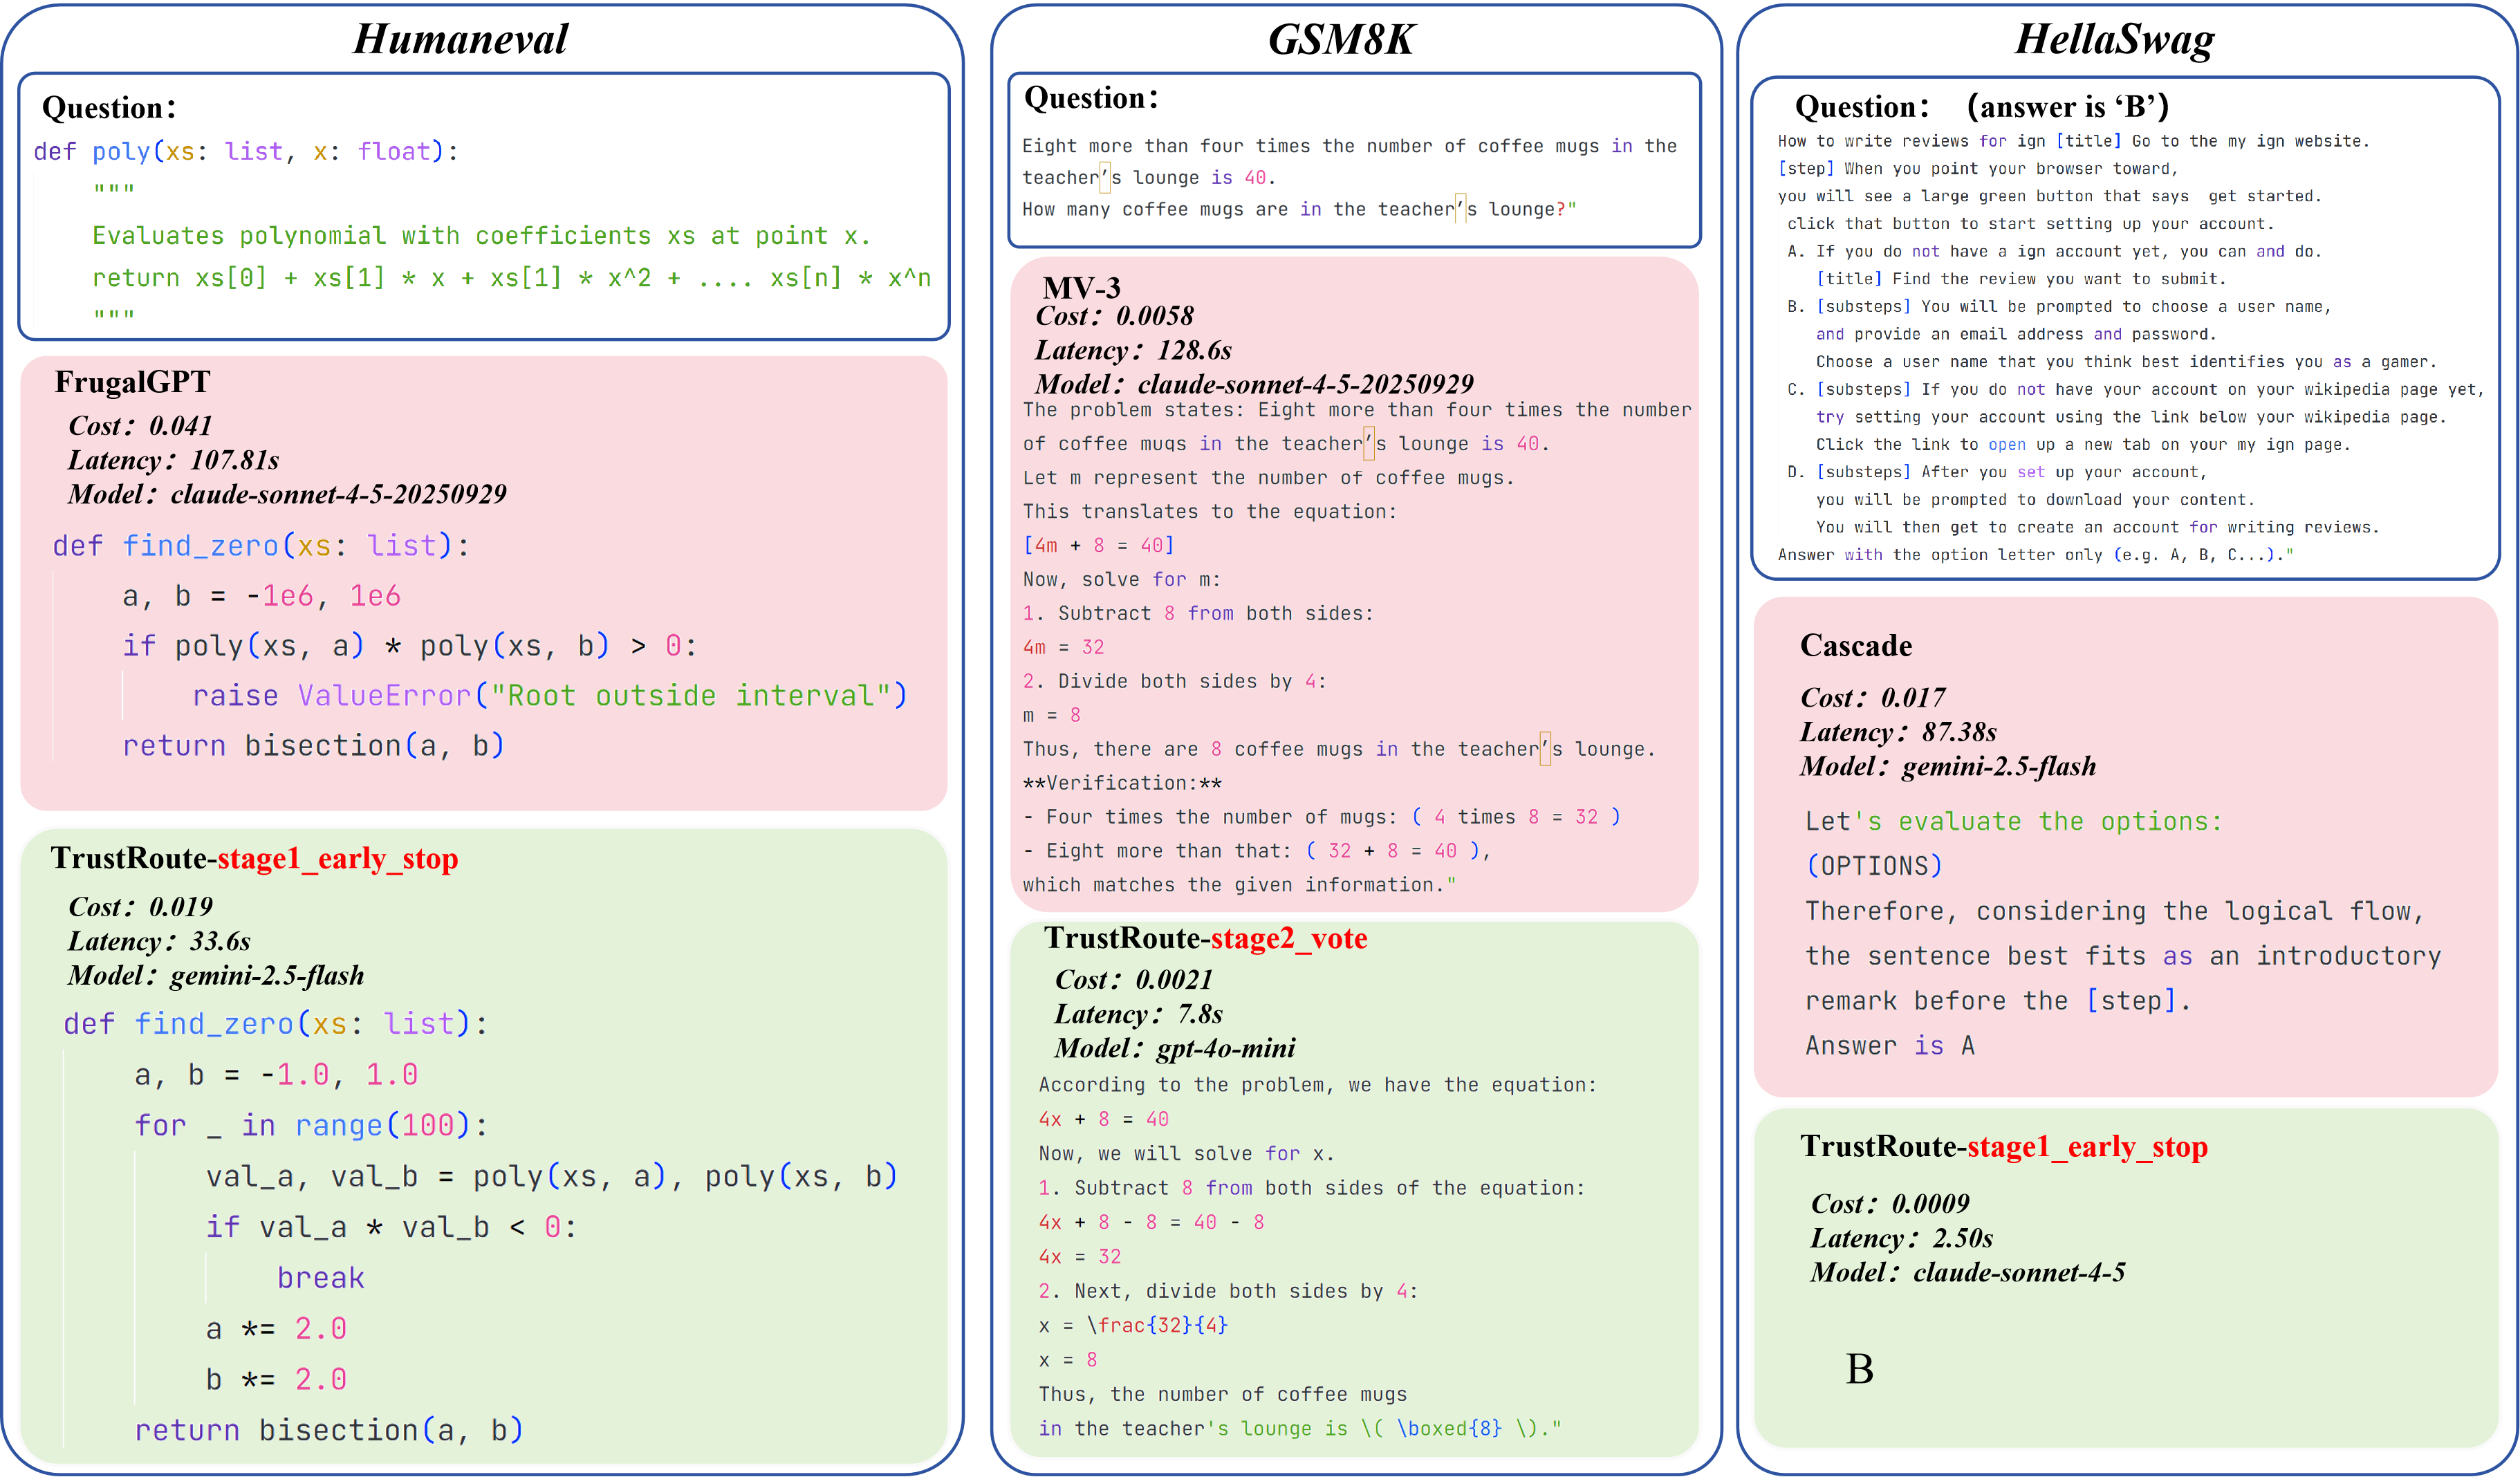
\includegraphics[width=\linewidth]{Pics/图片5.png}
    \caption{Case study on HumanEval, GSM8K, and HellaSwag.}
    \label{fig:case_study}
\end{figure}

In code generation, baselines like FrugalGPT inefficiently escalate to expensive models (e.g., Claude-Sonnet-4.5), incurring high costs (\$0.041) and latency (107.81s). In contrast, TrustRoute’s Stage-1 utilizes Gemini-2.5-Flash paired with sandbox execution (Fig. 1 Left). By triggering an early stop upon passing functional assertions, the system reduces costs to \$0.019 and latency to 33.6s. This confirms that execution feedback acts as a precise verification signal, eliminating the need for expensive models on solvable tasks.

For mathematical reasoning, the primary challenge is avoiding over-provisioning for simple tasks. As seen in Fig. 1 Center, while the MV-3 baseline correctly solved the problem, it exposed a massive inefficiency: it invoked the heavy-duty claude-sonnet-4-5 model for a straightforward linear equation, resulting in a disproportionate latency of 128.6s. In contrast, TrustRoute recognized the task complexity and routed it to the efficient gpt-4o-mini. This adaptive right-sizing achieved the same correct solution but with 94\% lower latency (7.8s) and 64\% lower cost (\$0.0021). This case highlights TrustRoute's ability to optimize the "cost of correctness"—avoiding the resource inefficiency of employing high-cost models for straightforward tasks.

In commonsense reasoning where execution is unavailable, TrustRoute leverages its Unsupervised Self-Adaptive Learning module to identify the optimal expert. While the Cascade baseline blindly cycled through models, accumulating massive latency of 87.38s and cost of \$0.017, TrustRoute utilized historical reputation scores to directly select claude-sonnet-4-5. As shown in Fig. 1 Right, this precision routing yielded the correct answer in just 2.50s with a total cost of \$0.0009, representing an 18x cost reduction. This confirms that learning which agent to trust via reputation is significantly more efficient than the brute-force trial-and-error approach of traditional cascading.

\section{Threats to Validity}
\label{sec:threats}

\paragraph{Internal validity.}
TrustRoute maintains online state (reputation) during inference, so results can depend on request order and transient API noise (latency spikes, occasional failures).
We mitigate this by isolating runs by \texttt{(dataset, seed)}, starting from clean caches, and reporting averages over three seeds (\S\ref{sec:exp_protocol}).
For executable tasks, outcomes may vary with sandbox settings (timeouts, runtime versions); we use a fixed sandbox/timeout policy across all methods.

\paragraph{Construct validity.}
Execution-based checks are an imperfect proxy for semantic correctness: unit tests (HumanEval/MBPP) are incomplete, and GSM8K correctness depends on deterministic answer extraction/normalization.
We follow standard benchmark protocols and apply the same extraction and execution pipeline to every method.
Our composite $J$ aggregates accuracy/cost/latency via per-dataset min--max normalization, so its absolute value depends on the compared method set; therefore we always report raw Accuracy/Cost/Latency alongside $J$ (Table~\ref{tab:main_results}).

\paragraph{External validity.}
Our model pool and pricing snapshot (Table~\ref{tab:model_pool}) reflect a particular set of commercial APIs and a specific time window; both model behavior and API pricing may change over time.
Moreover, the reported cost and latency metrics are based on specific commercial API pricing and network/runtime conditions at the time of experimentation (e.g., transient backend load and network jitter).
While we expect the \emph{relative} trends and comparisons across methods to be robust under similar settings, the \emph{absolute} cost/latency values may vary across deployments.

\paragraph{Conclusion validity.}
Black-box APIs introduce run-to-run variability (backend load, stochasticity).
We reduce this by multiple seeds and strict run isolation; nonetheless, we interpret improvements as evidence under the tested deployment conditions rather than universal guarantees.

\section{Discussion}
\label{sec:discussion}

Table~\ref{tab:main_results} highlights a key lesson for cost-aware deployment: issuing \emph{more} model calls does not necessarily
improve the reliability-per-dollar frontier. Large-sample self-consistency may slightly increase accuracy, but often inflates latency
(and sometimes cost) enough to hurt the overall trade-off. For example, on HumanEval, SC--10 is marginally more accurate than TrustRoute
(98.9\% vs.\ 97.7\%) but dramatically slower (46.81s vs.\ 8.24s), yielding a much lower J-Score (66.0 vs.\ 89.3).
A similar inefficiency appears for text-level voting: on ARC-Challenge, MV--3 reaches 96.9\% accuracy yet costs far more and runs much longer
($1.96\mathrm{e}{-3}$, 35.96s) than TrustRoute (97.3\%, $2.26\mathrm{e}{-4}$, 2.11s).
These gaps support our core claim that \textbf{Execution (PoT) can dominate Voting}: voting aggregates plausible-but-wrong outputs and
cannot separate uncompilable code, runnable-but-incorrect code, and truly correct solutions, whereas execution feedback acts as a precise
filter that enables early rejection and escalation only when needed.

Table~\ref{tab:main_results} also reveals a boundary case. On GSM8K, the cheap single-agent baseline is already near a strong operating
point, leaving limited headroom for escalation-based gains; in such near-saturated regimes, conservative triggering can add overhead without
proportional returns. Overall, TrustRoute benefits most when the base model has meaningful headroom and the verification signal is strong;
when verification is weaker, tighter escalation control and task-specific calibration become increasingly important.



\section{Related Work}

\textbf{LLM for Code Generation.} Recent LLM advances have reshaped automated code generation in software engineering.
Models such as Codex~\cite{chen2021codex} and CodeLlama~\cite{roziere2023codellama} leverage large-scale pretraining on code and text
to translate high-level specifications into executable programs, and are widely adopted in practice. However, they still lack intrinsic
verification: generation and correctness checking are typically separated, preventing models from incorporating execution feedback during
inference. TrustRoute addresses this gap by integrating execution-based verification~\cite{gao2022pal}.


\textbf{LLM Routing.} To reduce inference cost while maintaining output quality, recent work explores routing strategies that dynamically select among multiple models based on query characteristics. Representative approaches include Route LLM \cite{ong2024routellm}, TensorOpera \cite{stripelis2024tensoropera} Router, hybrid LLM \cite{ding2024hybrid}, and Intelligent Router for LLM Workloads \cite{jain2024intelligent}. These methods route requests using signals such as task complexity, model performance, and system load to reduce unnecessary computation. TrustRoute offers a training-free alternative with online adaptation, making it suitable for dynamic API environments.

\textbf{Automated Software Testing.} The use of large language models for automated software testing has attracted growing attention\cite{wang2023software}. LLMs have been applied to generating unit tests, assertions, and test suites\cite{schafer2023empirical}, as well as assisting bug detection and program verification. Most approaches generate tests from specifications or code and then execute them for downstream validation\cite{chen2023teaching,ni2023lever}. Our work aligns with this trend but inverts the pipeline: we use the test environment


\section{Conclusion}

We presented TrustRoute, a training-free framework for reliable code generation. By combining online reputation modeling with adaptive Program-of-Thought execution, we successfully optimized the trade-off between cost and reliability. Our extensive evaluation shows that TrustRoute achieves SOTA-level performance on reasoning tasks while significantly reducing costs.



\section*{Data Availability}
All code, datasets, and raw experimental results are available in our anonymous repository: \url{https://anonymous.4open.science/status/forAnonymize-CFFF}.

\bibliographystyle{ACM-Reference-Format}
\bibliography{sample-base}








\end{document}













% HellaSwag
\begin{table}[h]
\centering
\caption{Hyperparameter sensitivity on HellaSwag (dev set size $n=100$). $J$ is computed by min--max normalizing Acc/Cost/Lat within this table.}
\label{tab:ablate-hellaswag}
\small
\setlength\tabcolsep{4pt}
\begin{tabular}{lccc cccc}
\toprule
\multirow{2}{*}{\textbf{Variant}} &
\multicolumn{3}{c}{\textbf{Setting}} &
\multicolumn{4}{c}{\textbf{Metrics}} \\
\cmidrule(lr){2-4}\cmidrule(lr){5-8}
& $\tau_1$ & $\tau_2$ & $\mathbf{w}=(w_q,w_r,w_c)$
& Acc (\%) & Cost (USD) & Lat. (s) & $J$ \\
\midrule
Default              & 0.85 & 0.67 & (0.40,0.30,0.30) & 73.00 & $3.82\mathrm{e}{-5}$ & 1.451  & 65.8 \\
$\tau_1=0.75$        & 0.75 & 0.67 & (0.40,0.30,0.30) & 74.00 & $3.82\mathrm{e}{-5}$ & 2.159  & 65.4 \\
$\tau_1=0.95$        & 0.95 & 0.67 & (0.40,0.30,0.30) & 80.00 & $2.71\mathrm{e}{-3}$ & 14.475 & 33.3 \\
$\tau_2=1.00$        & 0.85 & 1.00 & (0.40,0.30,0.30) & 72.00 & $3.82\mathrm{e}{-5}$ & 1.481  & 66.9 \\
$w=(0.25,0.60,0.15)$ & 0.85 & 0.67 & (0.25,0.60,0.15) & 72.00 & $3.82\mathrm{e}{-5}$ & 1.480  & 66.9 \\
$w=(0.60,0.25,0.15)$ & 0.85 & 0.67 & (0.60,0.25,0.15) & 72.00 & $3.82\mathrm{e}{-5}$ & 1.478  & 66.9 \\
$w=(0.25,0.25,0.50)$ & 0.85 & 0.67 & (0.25,0.25,0.50) & 72.00 & $3.82\mathrm{e}{-5}$ & 1.657  & 65.9 \\
\bottomrule
\end{tabular}
\end{table}


% HumanEval
\begin{table}[t]
\centering
\caption{Hyperparameter sensitivity on HumanEval (dev set size $n=16$). $J$ is computed by min--max normalizing Acc/Cost/Lat within this table.}
\label{tab:ablate-humaneval}
\small
\setlength\tabcolsep{4pt}
\begin{tabular}{lccc cccc}
\toprule
\multirow{2}{*}{\textbf{Variant}} &
\multicolumn{3}{c}{\textbf{Setting}} &
\multicolumn{4}{c}{\textbf{Metrics}} \\
\cmidrule(lr){2-4}\cmidrule(lr){5-8}
& $\tau_1$ & $\tau_2$ & $\mathbf{w}=(w_q,w_r,w_c)$
& Acc (\%) & Cost (USD) & Lat. (s) & $J$ \\
\midrule
Default              & 0.85 & 0.67 & (0.40,0.30,0.30) & 87.50  & $8.58\mathrm{e}{-5}$ & 3.305 & 66.8 \\
$\tau_1=0.75$        & 0.75 & 0.67 & (0.40,0.30,0.30) & 87.50  & $8.11\mathrm{e}{-5}$ & 3.443 & 66.4 \\
$\tau_1=0.95$        & 0.95 & 0.67 & (0.40,0.30,0.30) & 100.00 & $1.31\mathrm{e}{-3}$ & 8.563 & 33.3 \\
$\tau_2=1.00$        & 0.85 & 1.00 & (0.40,0.30,0.30) & 81.25  & $8.15\mathrm{e}{-5}$ & 3.200 & 66.7 \\
$w=(0.25,0.60,0.15)$ & 0.85 & 0.67 & (0.25,0.60,0.15) & 87.50  & $9.40\mathrm{e}{-5}$ & 3.616 & 64.9 \\
$w=(0.60,0.25,0.15)$ & 0.85 & 0.67 & (0.60,0.25,0.15) & 87.50  & $7.66\mathrm{e}{-5}$ & 3.214 & 67.3 \\
$w=(0.25,0.25,0.50)$ & 0.85 & 0.67 & (0.25,0.25,0.50) & 81.25  & $7.93\mathrm{e}{-5}$ & 3.178 & 67.0 \\
\bottomrule
\end{tabular}
\end{table}


% MBPP
\begin{table}[t]
\centering
\caption{Hyperparameter sensitivity on MBPP (dev set size $n=37$). $J$ is computed by min--max normalizing Acc/Cost/Lat within this table.}
\label{tab:ablate-mbpp}
\small
\setlength\tabcolsep{4pt}
\begin{tabular}{lccc cccc}
\toprule
\multirow{2}{*}{\textbf{Variant}} &
\multicolumn{3}{c}{\textbf{Setting}} &
\multicolumn{4}{c}{\textbf{Metrics}} \\
\cmidrule(lr){2-4}\cmidrule(lr){5-8}
& $\tau_1$ & $\tau_2$ & $\mathbf{w}=(w_q,w_r,w_c)$
& Acc (\%) & Cost (USD) & Lat. (s) & $J$ \\
\midrule
Default              & 0.85 & 0.67 & (0.40,0.30,0.30) & 81.08 & $6.71\mathrm{e}{-5}$ & 2.905  & 66.0 \\
$\tau_1=0.75$        & 0.75 & 0.67 & (0.40,0.30,0.30) & 78.38 & $6.65\mathrm{e}{-5}$ & 2.677  & 67.2 \\
$\tau_1=0.95$        & 0.95 & 0.67 & (0.40,0.30,0.30) & 83.78 & $3.18\mathrm{e}{-3}$ & 12.904 & 33.3 \\
$\tau_2=1.00$        & 0.85 & 1.00 & (0.40,0.30,0.30) & 78.38 & $6.61\mathrm{e}{-5}$ & 2.674  & 67.2 \\
$w=(0.25,0.60,0.15)$ & 0.85 & 0.67 & (0.25,0.60,0.15) & 78.38 & $6.58\mathrm{e}{-5}$ & 2.856  & 66.8 \\
$w=(0.60,0.25,0.15)$ & 0.85 & 0.67 & (0.60,0.25,0.15) & 81.08 & $6.69\mathrm{e}{-5}$ & 2.771  & 66.1 \\
$w=(0.25,0.25,0.50)$ & 0.85 & 0.67 & (0.25,0.25,0.50) & 78.38 & $6.58\mathrm{e}{-5}$ & 2.699  & 67.1 \\
\bottomrule
\end{tabular}
\end{table}


% MMLU
\begin{table}[t]
\centering
\caption{Hyperparameter sensitivity on MMLU (dev set size $n=100$). $J$ is computed by min--max normalizing Acc/Cost/Lat within this table.}
\label{tab:ablate-mmlu}
\small
\setlength\tabcolsep{4pt}
\begin{tabular}{lccc cccc}
\toprule
\multirow{2}{*}{\textbf{Variant}} &
\multicolumn{3}{c}{\textbf{Setting}} &
\multicolumn{4}{c}{\textbf{Metrics}} \\
\cmidrule(lr){2-4}\cmidrule(lr){5-8}
& $\tau_1$ & $\tau_2$ & $\mathbf{w}=(w_q,w_r,w_c)$
& Acc (\%) & Cost (USD) & Lat. (s) & $J$ \\
\midrule
Default              & 0.85 & 0.67 & (0.40,0.30,0.30) & 83.00 & $2.45\mathrm{e}{-4}$ & 1.973 & 66.9 \\
$\tau_1=0.75$        & 0.75 & 0.67 & (0.40,0.30,0.30) & 85.00 & $2.91\mathrm{e}{-4}$ & 2.082 & 66.2 \\
$\tau_1=0.95$        & 0.95 & 0.67 & (0.40,0.30,0.30) & 87.00 & $2.20\mathrm{e}{-3}$ & 5.725 & 33.3 \\
$\tau_2=1.00$        & 0.85 & 1.00 & (0.40,0.30,0.30) & 82.00 & $1.92\mathrm{e}{-4}$ & 1.850 & 66.7 \\
$w=(0.25,0.60,0.15)$ & 0.85 & 0.67 & (0.25,0.60,0.15) & 84.00 & $2.24\mathrm{e}{-4}$ & 1.940 & 67.3 \\
$w=(0.60,0.25,0.15)$ & 0.85 & 0.67 & (0.60,0.25,0.15) & 83.00 & $2.37\mathrm{e}{-4}$ & 1.968 & 67.0 \\
$w=(0.25,0.25,0.50)$ & 0.85 & 0.67 & (0.25,0.25,0.50) & 84.00 & $2.45\mathrm{e}{-4}$ & 1.889 & 67.1 \\
\bottomrule
\end{tabular}
\end{table}


% Winogrande
\begin{table}[t]
\centering
\caption{Hyperparameter sensitivity on Winogrande (dev set size $n=126$). $J$ is computed by min--max normalizing Acc/Cost/Lat within this table.}
\label{tab:ablate-winogrande}
\small
\setlength\tabcolsep{4pt}
\begin{tabular}{lccc cccc}
\toprule
\multirow{2}{*}{\textbf{Variant}} &
\multicolumn{3}{c}{\textbf{Setting}} &
\multicolumn{4}{c}{\textbf{Metrics}} \\
\cmidrule(lr){2-4}\cmidrule(lr){5-8}
& $\tau_1$ & $\tau_2$ & $\mathbf{w}=($(w_q,w_a,w_h)$)$
& Acc (\%) & Cost (USD) & Lat. (s) & $J$ \\
\midrule
Default              & 0.85 & 0.67 & (0.40,0.30,0.30) & 69.05 & $1.52\mathrm{e}{-5}$ & 1.321 & 66.4 \\
$\tau_1=0.75$        & 0.75 & 0.67 & (0.40,0.30,0.30) & 72.22 & $1.52\mathrm{e}{-5}$ & 1.255 & 67.0 \\
$\tau_1=0.95$        & 0.95 & 0.67 & (0.40,0.30,0.30) & 91.27 & $1.19\mathrm{e}{-3}$ & 3.870 & 33.3 \\
$\tau_2=1.00$        & 0.85 & 1.00 & (0.40,0.30,0.30) & 73.02 & $1.52\mathrm{e}{-5}$ & 1.331 & 66.4 \\
$w=(0.25,0.60,0.15)$ & 0.85 & 0.67 & (0.25,0.60,0.15) & 72.22 & $1.52\mathrm{e}{-5}$ & 1.323 & 66.4 \\
$w=(0.60,0.25,0.15)$ & 0.85 & 0.67 & (0.60,0.25,0.15) & 70.63 & $1.52\mathrm{e}{-5}$ & 1.256 & 67.0 \\
$w=(0.25,0.25,0.50)$ & 0.85 & 0.67 & (0.25,0.25,0.50) & 71.43 & $1.52\mathrm{e}{-5}$ & 1.300 & 66.5 \\
\bottomrule
\end{tabular}
\end{table}